\documentclass[ a4paper,
                oneside,
                toc=bibliography,
                toc=listof
                ]{scrbook}

\usepackage[ngerman]{babel} % If the thesis is in English
\usepackage {longtable}
\usepackage{tikz}
\usetikzlibrary{positioning,calc}
\usepackage{tikz-uml}
\usetikzlibrary{positioning, arrows.meta}
\usepackage{geometry}
\usetikzlibrary{matrix}
\usetikzlibrary{fit,matrix,shapes.geometric}
\usetikzlibrary{positioning, shapes, arrows, decorations.pathreplacing}
\usepackage[table]{xcolor}
\usepackage{nicematrix,booktabs,tikz}
\usepackage{harveyballs}
\usepackage{tabularx}
\usepackage{pgfgantt}
\usepackage{pgf-umlsd}
\usepackage[T1]{fontenc}
\usepackage[utf8]{inputenc}
\usepackage{amsmath}


%\usepackage[english, ngerman]{babel} % If the thesis is in German


% This class does the ISW styling for you (together with scrbook).
%
% It handles the following:
% - Proper input and font encoding (Just type, don't care about the LaTeX compiler you use or how to type German umlauts)
% - Fonts with ligatures and kerning (Tex Gyre fonts are used, part of every LaTeX installation, text is nice to read)
% - Bibliography styling for biblatex (declare your bibliography file and you are ready to go)
% - Provide command for title page (\makeISWtitle) and declaration of originality ( \declarationOfOriginality)
% - Loads packages "biblatex" and "graphics"
\usepackage[
    type=study, % master, bachelor, bachelorproject
]{iswthesis}

%Path to .bib-File(s) for BibLatex
\addbibresource{bibliography.bib}
% \addbibresource{someOtherBibFile}

\author{Lukas Schlotter}
\placeOfBirth{Stuttgart}
\major{Mechatronik}
\title{Konzeption und Implementierung einer Diagnoseschnittstelle zwischen Industrieroboter und Anlagensteuerung}
\titleTranslated{Design and Implementation of a Diagnostic Interface between Industrial Robot and Control System}
\matrnr{3668915}
\date{\today}
\supervisor{Dr.-Ing. Andreas Wolf, Dipl.-Ing. Daniel Knauss}
\professor{Prof. Dr.-Ing. Alexander Verl}

\begin{document} 
    \frontmatter
    \makeISWtitle
    
    \cleardoublepage
	\setcounter{page}{1} % start at page (i) after title page
    %\declarationOfOriginality

    % Kurzfassung/Abstract
    
    \cleardoublepage
    \tableofcontents
    

    \mainmatter
    
    \chapter{Einleitung}

    \section{Motivation}
    Roboter sind in unserer Welt nicht mehr wegzudenken. In unterschiedlichsten Industrien verrichten sie zuverlässig ihre Arbeit und machen eine Produktion auch in Hochlohnländern wirtschaftlich. Ihre Arbeitsleistung ist konstant, fehlerfrei und präzise. In der Lebensmittel Industrie gelten besondere Hygiene-Anforderungen, denen Roboter der Stäubli-AG gerecht werden. Mit ihnen können beispielsweise Wiener-Würste verpackt werden. Um eine solche anspruchsvolle Aufgabe zu bewältigen, entwickelt die "robomotion GmbH" komplexe Automatisierungslösungen ganz individuell nach den Kundenbedürfnissen. Eine solche Anlage setzt nicht neben einem oder mehreren Robotern aus vielen weiteren Komponenten, wie z.b. einem Förderband, der zentralen Steuerung durch die SPS, sowie einem PC für die Datenverwertung, sowie als Schnittstelle zum Bediener zusammen. Um ein gutes Zusammenspiel aller Komponenten zu gewährleisten, ist eine Kommunikation zwischen ihnen von großer Bedeutung. Dies ist besonders wichtig, da die Datenmenge in der heutigen Zeit kontinuierlich wächst und Kunden ein großes Interesse an Informationen über ihre Anlagen und Roboter haben. 
	\section{Zielsetzung / Aufgabenstellung}
	In der robomotion GmbH sollen Stäubli-Roboter neu eingeführt und in das bestehende Anlagensteuerungskonzept integriert werden. Hierzu soll eine bidirektionale Kommunikationsschnittstelle zwischen der Anlage und dem Roboter entworfen und implementiert werden. Diese setzt sich aus zwei getrennten Einheiten zusammen. Eine Feldbus-Verbindung muss Befehle von der Anlagen-SPS zum Roboter übertragen. Darüber hinaus müssen Fehlermeldungen und Prozessdaten des Roboters zur Anlagenvisualisierung und Kameradaten von der Anlagenvisualisierung zum Roboter übertragen werden. Die Visualisierung und Verwertung dieser Daten erfolgt jedoch nicht in der SPS, sondern in einem auf Windows laufenden .NET basierten Programm. Aus diesem Grund muss eine zweite Kommunikationsverbindung zwischen Roboter und Anlage mit Hilfe von TCP/IP konzeptioniert, entworfen und implementiert werden. Der Schwerpunkt dieser Arbeit liegt auf der TCP/IP-Verbindung.\\
	Im Rahmen dieser Arbeit, soll sowohl der Feldbus, als auch die TCP/IP-Verbindung konzeptioniert werden. Das Programm für den Roboter, sowie eine sogenannte WPF-Anwendung für das Windows-Betriebssystem sollen konzeptioniert, entworfen und implementiert werden. Eine Oberfläche soll dem Bediener die Fehlermeldungen des Roboters anzeigen. Ein Praxistest soll abschließend das entwickelte Gesamtsystem validieren. Darüber hinaus sollen die Potentiale, welche durch die zur Verfügung stehenden Daten entstehen, sowie mögliche Verwendungsszenarien aufgezeigt werden.
	
	\section{Methodik und Vorgehensweise}
	Die Verwendung geeigneter Methoden und eines strukturierten Vorgehens sind entscheidend für eine erfolgreiche Umsetzung des Projektes. Durch ein Vorgehensmodell wird eine effiziente Arbeitsweise gefördert und durch eine Terminplanung eine zeitgerechte Fertigstellung sichergestellt. Methoden und Werkzeuge, wie bspw. ein morphologischer Kasten oder ein Harvey-Diagramm erleichtern es neue Lösungsansätze zu finden und faktenbasierte Entscheidungen zu treffen. \cite{SoftwaretechnikBroy} \cite{ISWLeitfaden} \\
	\textbf{Vorgehensweise}\\
	Die Vorgehensweise lehnt sich an Sommerville \cite{Sommerville} und an den ISW-Leitfaden \cite{ISWLeitfaden}. Da es sich in dieser Arbeit um kein reines Softwareprojekt handelt, sondern ebenso mechatronische Komponenten, wie der Roboter und die Kommunikationsschnittstelle enthalten sind erfolgt eine Anpassung der Vorgehensweise an die gegebenen Randbedingungen. Hieraus ergibt sich folgende Abfolge:\\
	\begin{itemize}
		\item \textbf{Recherche zu Grundlagen und Stand der Technik:} Zu Beginn soll zur Einarbeitung eine Recherche zu den Grundlagen von Feldbussen und TCP/IP erfolgend. Ebenso muss eine Recherche zum Stand der Technik des Roboters und der Anlagensteuerungskonzept von robomotion erfolgen. In der Literatur soll  nach gängigen Umsetzungen von TCP/IP-Verbindungen im Kontext von Robotern gesucht werden.
		\item \textbf{Detaillierung der Anforderungen:} Die grobe Aufgabenstellung soll detailliert und in ein Lastenheft überführt werden.
		\item \textbf{Konzeptionierung:} Hier soll die Feldbus-Verbindung zwischen Roboter und SPS konzeptioniert werden. Vorallem ist die TCP/IP-Kommunikation zu konzeptionieren und Entscheiden bezüglich Nachrichtenaufbau und Kommunikationsablauf festzulegen. Ebenso sollen die zu übertragenden Daten gewählt werden.
		\item \textbf{Softwaredesign:} In diesem Rahmen soll ein Systementwurf der Software für den Stäubli-Roboter und vorallem der WPF-Anwendung erfolgen. Die Architektur, sowie Lösungsbausteine, wie Softwarebibliotheken müssen festgelegt werden. Softwarekomponenten entweder hier oder in der Konzeptionierung festlegen. Wenn man es hier macht, hat man ein Teil der Spezifikation/Konzeption mit hierdrin.
		\item \textbf{Softwareimplementierung:} Die zuvor konzeptionierte und entworfene Software muss in einen Source-Code überführt werden. Bei der Programmierung ist auf verständliche Kommentierung zu achten und eine Verwaltung soll mit Hilfe eines Source-Code-Verwaltungs-Programm erfolgen.
		\item \textbf{Validierung:} Durch eine abschließende Validierung ist das System unter Realbedingungen zu testen. Dies soll ein Funktionstest beinhalten, um zu überprüfen, dass alle Funktionen ihre Aufgaben erfüllen. Fehlertests prüfen die Robustheit des Systems. Hierzu werden bewusst besondere Situationen oder Störungen herbeigeführt um die Fehlertoleranz des Systems zu überprüfen und sicherzustellen, dass das System nicht abstürzt. \cite{ISWLeitfaden} \cite{Sommerville}
	\end{itemize}
	Die schriftliche Ausarbeitung folgt ebenso diese Vorgehensweise. Eine vollständige Aufführung der Implementierung, welche sich durch den gesamten Quell-Code darstellt ist nicht sinnvoll. Aus diesem Grund wird die Implementierung mit in das Kapitel Softwaredesign integriert und lediglich besonders erwähnenswerte und für das Verständnis wichtige kurze Code-Abschnitte aufgezeigt. Abgerundet wird die Arbeit durch ein Fazit und einem Ausblick.\\
	\textbf{Terminplanung}\\
	Für eine fristgerechte Fertigstellung und ein strukturiertes Vorgehen ist es wichtig zu Beginn eine Terminplanung durchzuführen. Hierzu kommt ein Gantt-Diagramm zum Einsatz (vgl. Tabelle \ref{tab:Gantt}). Die horizontalen Balken stellen die einzelnen Arbeitspakete und deren Zeitumfang dar. Meilensteine, sind wichtige Projekt-(Zwischen)-Ziele mit einer Zeitdauer Null und werden mit einer Raute dargestellt. \cite{ISWLeitfaden}\\
	Um frühzeitig Umsetzungsschwierigkeiten zu erkennen und Lösungskonzepte zu testen soll parallel zu der Konzeptionierung ein Softwareprototyp mitgeführt werden. Ebenso soll die Datenübertragung an der Hardware möglichst früh im Projektverlauf getestet werden. Dadurch kann die entworfene Verbindung, sowie die Softwarekonzepte zwischenzeitlich abgesichert werden. Dies verhindert, dass erst in der Implementierung sich herausstellt, dass grundlegende Funktionalitäten nicht funktionieren. 
	
	\begin{table}
		\centering
		\caption{Terminplanung mit Gantt-Diagramm}
		\label{tab:Gantt}
		\begin{ganttchart}[
			vgrid={*{12}{gray, dotted}, *1{black, dashed}},
			bar label node/.append style={
				align=left,
				text width=width("Einarbeitung und Literatur ")},
				bar/.append style={fill=blue!50},
				milestone/.append style={fill=orange},
				milestone label node/.append style={align=left, text width=width("Einarbeitung und Literatur ")},
			]{1}{19}
			\gantttitle{2023}{13} \gantttitle{2024}{6} \\
			\gantttitlelist{40,41,42,43,44,45,46,47,48,49,50,51,52,1,2,3,4,5,6}{1} \\
			\ganttbar{Einarbeitung und Literatur}{1}{4} \\
			\ganttbar{Anforderungsanalyse}{4}{4} \\
			\ganttbar{Konzeptionierung Feldbus}{5}{5} \\
			\ganttbar{Konzeptionierung TCP/IP}{6}{9} \\
			\ganttbar{Konzeptionierung WPF}{8}{9} \\
			\ganttmilestone{M: Fertiges Konzept}{9}\\
			\ganttbar{Softwaredesign}{10}{12} \\
			\ganttbar{Softwareimplementierung}{13}{15} \\
			\ganttmilestone{M: Fertigstellung Code}{15} \\
			\ganttbar{Validierung und Testing}{16}{17} \\
			\ganttmilestone{M: Validiertes System}{17}\\
			\ganttbar{Dokumentation}{12}{19}\\
			\ganttmilestone{M: Präsentation und Abgabe}{19}
		\end{ganttchart}
	\end{table}

	\chapter{Grundlagen und Stand der Technik}
	
	\section{Feldbusse}
	Maschinen und Anlagen verfügen über eine Vielzahl an Sensoren und Aktoren. Diese werden klassisch über Parallelverdrahtung an die Ein-und Ausgänge der SPS angeschlossen. Ein Feldbus ermöglicht es dagegen die Sensoren und Aktoren an einzelne aktive Verteilerboxen anzuschließen. Die Verteilerboxen werden wiederum mit einem Feldbus untereinander und mit der SPS verbunden. Dies ermöglicht eine Dezentralisierung, was den Schaltschrank vereinfacht, die Energieeffizient steigert und die Flexibilität bezüglich Änderungen erhöht. Der Übergang von der Parallelverdrahtung zu der Fehlbusverdrahtung ist mit den Zwischenschritt von passiven Verteilerboxen nachfolgend dargestellt (vgl. Abbildung \ref{fig:Parallel_vs_Feldbus}). Bei der Feldbus Anschaltung wird meist wie in der Abbildung dargestellt eine Linien-Struktur verwendet. Alternativen sind die Stern-, Ring- oder Baum-Struktur. \cite{hering2012elektrotechnik}
	\begin{figure}[!ht]
		\centering
		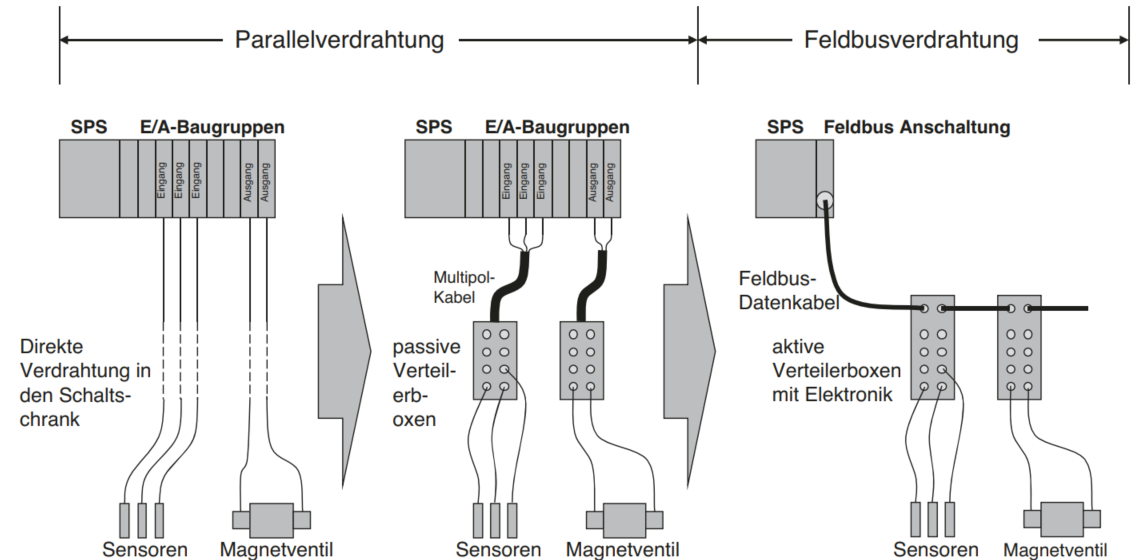
\includegraphics[width=1.0\linewidth]{./images/Parallelverdrahtung_Feldbus.png}
		\caption{Übergang Parallelverdrahtung zu Feldbussen \cite{hering2012elektrotechnik}}
		\label{fig:Parallel_vs_Feldbus}
	\end{figure}\\
	Es haben sich Feldbusse von vielen namhaften Herstellern etabliert. Mittlerweile werden diese Standard-Feldbusse immer weiter von Ethernet basierenden Feldbussen (auch Industrial Ethernet genannt) abgelöst, da diese vor allem Vorteile bezüglich der Übertragungsgeschwindigkeit aufweisen. Die Marktaufteilung aus dem Jahr 2021 ist nachfolgend abgebildet, wobei eine weitere Zunahme der Marktanteile von den Ethernet basierenden Feldbussen zu erwarten ist (vgl. Abbildung \ref{fig:Marktanteil_Feldbus}). \cite{hering2012elektrotechnik} \cite{Marktanteile_HMS}\\
	\begin{figure}[!ht]
		\centering
		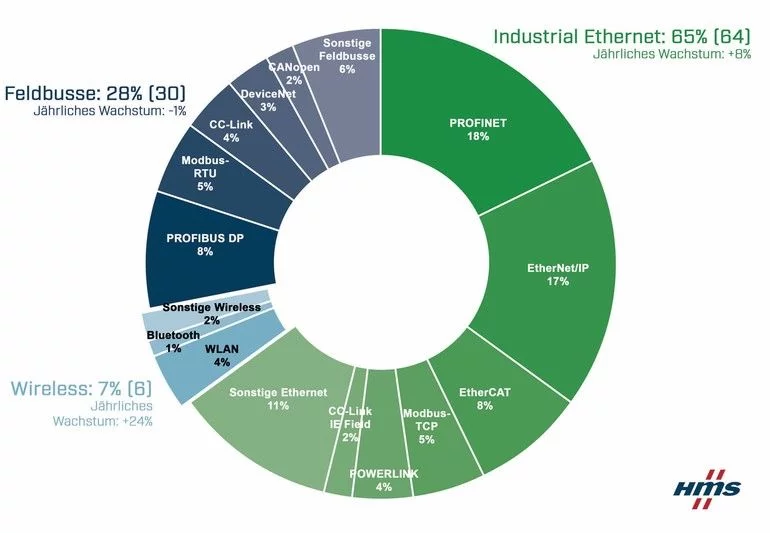
\includegraphics[width=1.0\linewidth]{./images/HMS__Marktanteile_industrielle_Netzwerke.png}
		\caption{Marktanteile Feldbusse und Industrial Ethernet  \cite{Marktanteile_HMS}}
		\label{fig:Marktanteil_Feldbus}
	\end{figure}\\
	\label{sec:Feldbus}
	\subsection{Standard-Feldbusse}
	In der Anlagentechnik und der Robotik ist die sofortige zuverlässige Datenübertragung unter anderem aus Gründen der Sicherheit essentiell. Feldbusse sind daher echtzeitfähig. Die Echtzeitfähigkeit besagt, dass die Daten innerhalb einer sehr kurzen festgelegten Zeitspanne unabhängig von äußeren Einflüssen übertragen werden müssen. Durch die harte Echtzeit, ist im Gegensatz zur weichen Echtzeit zusätzlich definiert, dass die Daten mit einem absoluten Determinismus übertragen werden müssen. Bei der weichen Echtzeit verlieren die Daten lediglich an Nutzen bei verspätetem Eintreffen, bei der harten Echtzeit werden sie komplett nutzlos. Aus diesem Grund müssen bei der harten Echtzeit 100 \% der Daten innerhalb der definierten Zeit übertragen werden, was insbesondere bei sicherheitsrelevanten Funktionen von Relevanz ist. \cite{dopatka2008framework} \cite{Echtzeit} \\
	Im folgenden sollen ein paar gängige Feldbusse kurz erwähnt und erläutert werden.\\
	\textbf{Profibus} wird von dem Dachverband "Profibus \&Profinet" International" verwaltet, um die Interessen der Nutzer einzubringen. Neben dem Profibus auf Feldbus-Ebene (auch Profibus-DP genannt) existiert eine weitere Variante auf Zellensteuerungs-Ebene und eine auf Prozess-Automatisierungs-Ebene. Als Übertragungstechnik dient der sogenannte RS485-Standard mit einer Zweidrahtleitung. Die Datentransferrate von Profibus beträgt bis zu 12 MBit/s. Speicherprogrammierbare Steuerungen von Siemens setzen häufig Profibus ein.  \cite{hering2012elektrotechnik}\\
	\textbf{CAN-Bus} wurde ursprünglich für die Automobil-Industrie entwickelt und kommt dort heute noch zum Einsatz. Darüber hinaus, nahm die Verbreitung in der Anlagensteuerung zu. Möglich sind Datentransferraten von bis zu 1 MBit/s. Als Übertragungsmedium dient eine Zweidrahtleitung.  CAN-Bus zeichnet sich durch eine besonders hohe Datensicherheit, also eine hohe Zuverlässigkeit bei der Datenübertragung aus, weshalb er in der Medizintechnik und Robotik hohen Zuspruch findet. \cite{hering2012elektrotechnik}\\
	\textbf{DeviceNet} basiert auf CAN und ist eine Entwicklung des nordamerikanischen Herstellers "Rockwell Automation". Die Datenübertragungsrate beträgt bis zu 500 kBit/s und die Spannungsversorgung, sowie die Datenkommunikation können über ein Kabel erfolgen. \cite{hering2012elektrotechnik}\\
	\textbf{CC-Link} stellt eine Entwicklung des Unternehmen Mitsubishi dar. Verwaltet wird das Protokoll von einer Anwenderorganisation ähnlich zu Profibus. Die maximale Übertragungsrate beträgt 10 MBit/s und als Übertragungsmedium dient eine dreiadrige Leitung. \cite{hering2012elektrotechnik}\\
	\label{subsec:StandardFeldbus}
	\subsection{Ethernet basierende Feldbusse}
	Ethernet basierende Feldbusse, häufig auch als "Industrial Ethernet" bezeichnet, ermöglichen deutlich höhere Übertragungsraten als Standard-Feldbusse. Daher nimmt deren Verbreitung ständig zu und lösen in vielen Bereichen den Standard-Feldbus ab. \cite{hering2012elektrotechnik}\\
	\textbf{Ethernet-Technologie}\\
	Ethernet ist einer von mehreren Standards für die lokale Netzwerkverbindung mittels LAN-Technologie. Sie ist im IEE 802-3- Standard (Institute of Electrical and Electronis Engineers) genormt. Der Aufbau eines Ethernet-Telegramms ist nachfolgend abgebildet (vgl. Abbildung \ref{fig:EthernetTelegramm}). Die Adressierung erfolgt mittels MAC-Adresse oder IP-Adresse (mehr hierzu in Kapitel \ref{sec:TCP/IP}). \cite{riggert2002rechnernetze}\\
	\begin{figure}[!ht]
		\centering
		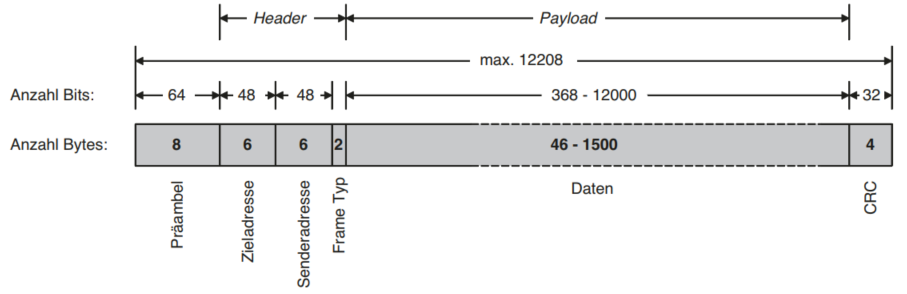
\includegraphics[width=1.0\linewidth]{./images/Ethernet-Telegram.png}
		\caption{Telegramm-Aufbau Ethernet \cite{hering2012elektrotechnik}}
		\label{fig:EthernetTelegramm}
	\end{figure}
	Verschiedene Geräte sind an das Übertragungsmedium angeschlossen und teilen sich dieses. Man spricht von einem Multi-Master-Bus, da jedes Gerät selbständig die Initative ergreifen kann, um Nachrichten zu senden. Damit jedes Gerät kommunizieren kann und dabei Sendekonflikte vermieden werden kommt bei Ethernet der CSMA/CD-Mechanismus zum Einsatz. CSMA/CD steht für "Carrier Sense Multiple Access with Collision Detection" und ermöglicht einen mehrfachen Zugriff (Muliple Access) auf das Übertragungsmedium. \cite{hering2012elektrotechnik} \cite{riggert2002rechnernetze}
	\begin{itemize}
		\item \textbf{Carrier Sense:} Es überwacht, dass das Übertragungsmedium nicht durch ein anderes Gerät belegt ist. Erst nachdem das Medium als frei erkannt wird, erfolgt nach einer kurzen Wartezeit die Übertragung. Während des Sendens, wird das Medium weiterhin auf Kollisionen abgehört.
		\item \textbf{Multiple Access:} Es besagt, dass alle Geräte gleichberechtigt auf das Übertragungsmedium zugreifen können.
		\item \textbf{Collision Detection:} Wenn mehrere Geräte zur gleichen Zeit das Übertragungsmedium als frei erkennen kommt es zur Überlagerung, da mehrere Geräte gleichzeitig beginnen zu senden. Dies wird als Kollision bezeichnet und es kommt zur Signalverfälschung durch Überlagerung. Da jeder Sender das Übertragungsmedium während des Sendevorgangs überwacht wird die Kollision direkt erkannt. Dasjenige Gerät, welches die Kollision erkennt, informiert alle anderen Geräte mittels eines Signales über die aufgetretene Kollision und fordert diese zur Unterbrechung jeglicher Übertragung auf. \\
		Danach warten die Geräte eine zufällige Zeitspanne ab und versuchen das Senden erneut. \cite{riggert2002rechnernetze}
	\end{itemize}
	Durch die Kollisionen kommt es zu nicht vorhersehbaren Wartezeiten im Sendeprozess. Daher handelt es sich um ein nicht deterministisches Zugriffsverfahren. Ethernet mit CSMA/CD ist nicht echtzeitfähig, was wie bereits in Kapitel \ref{subsec:StandardFeldbus} erwähnt, zu Problem bei Automatisierungsanlagen führen kann.\\
	Um die Ethernet-Technologie dennoch in der Automatisierung zu nutzen, haben die Hersteller verschiedene Echtzeitprotokolle entwickelt, um Ethernet echtzeitfähig zu machen. Beispielsweise wird die Methodik CSMA/CD außer Kraft gesetzt und stattdessen durch sogenanntes Pooling oder ein Zeitscheibenverfahren ersetzt. Jeder Hersteller geht hier jedoch seinen eigenen Weg.	Bekannte Ethernet basierende Feldbusse sind Profinet, Ethernet/IP, EtherCAT und Sercos III.
	EtherCAT ist eine Technologie des Herstellers "Beckhoff", dessen SPS im Rahmen dieses Projektes zum Einsatz kommt. Aus diesem Grund ist EtherCAT die bevorzugte Technologie und wird im Rahmen dieser Arbeit näher erläutert. \cite{ethercat} \cite{riggert2002rechnernetze}\
	\\
	Weiterhin ist zu beachten, dass die Netzwerktopologie sich bei den Ethernet basierenden Feldbussen häufig von den Standard-Feldbussen unterscheidet. Während bei den Standard-Feldbussen die Ansteuerung vorwiegend in der Linienstruktur erfolgt, wird bei der Ethernet Anschaltung oft eine Sternstruktur mit einem Switch eingesetzt (vgl. Abbildung \ref{fig:TopologieEthernet}).
	\begin{figure}[!ht]
		\centering
		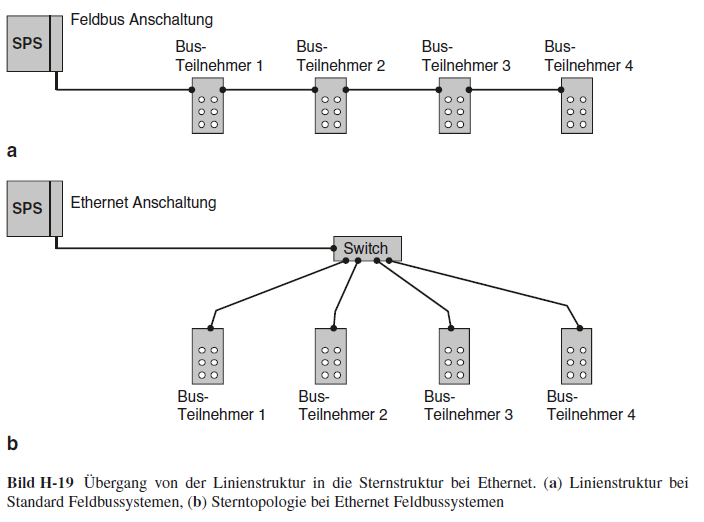
\includegraphics[width=1.0\linewidth]{./images/Feldbus vs Ethernet Anschaltung.png}
		\caption{Topologie: oben Standard-Feldbus, unten Ethernet basierender Feldbus \cite{hering2012elektrotechnik}}
		\label{fig:TopologieEthernet}
	\end{figure}\\
	Der Ethernet Switching Hub, abgekürzt als Switch erlernt beim Einschalten an welchen Ports  Teilnehmer angeschlossen sind. Der Switch leitet ein Datentelegramm eindeutig vom Sender zum Empfänger. Dadurch werden von dem Telegramm nicht betroffene Teilnehmer und Ethernet-Segmente nicht unnötig belastet und Kollisionen vermieden. Das Weiterschalten erfolgt auf Basis der Sende- und Ziel-Adresse, welche im Ethernet-Telegramm hinterlegt ist. \cite{hering2012elektrotechnik} \\
	\textbf{EtherCAT} \\
	Wie bereits erwähnt setzen viele Hersteller auf das Zeitscheibenverfahren oder Pooling, um EtherNet echtzeitfähig zu machen. Der Zeitverzug ist hierbei jedoch implementierungsabhängig und kann durch erforderliche technische Komponenten am Bus weiter steigen. Um dies zu verhindern setzt EtherCAT auf einen anderen Lösungsansatz. Im Gegensatz zu anderen Verfahren sollen Daten nicht mehr empfangen, interpretiert und dann wieder weiterversendet werden. Stattdessen setzt EtherCAT auf sogenannte FMMU (Fieldbus Memory Management Unit) in allen E/A-Klemmen. Diese FMMU entnimmt nur die relevanten Daten vom Bus, sodass die Telegramme mit einer Verzögerung von nur wenigen Nanosekunden weiterlaufen können. Zum Versenden werden Daten in die durchlaufenden Telegramme eingefügt, sodass es auch hier zu kaum einer Verzögerung kommt. Dieses Prinzip ist nachfolgend dargestellt (vgl. Abbildung \ref{fig:EtherCAT}).
	\begin{figure}[!ht]
		\centering
		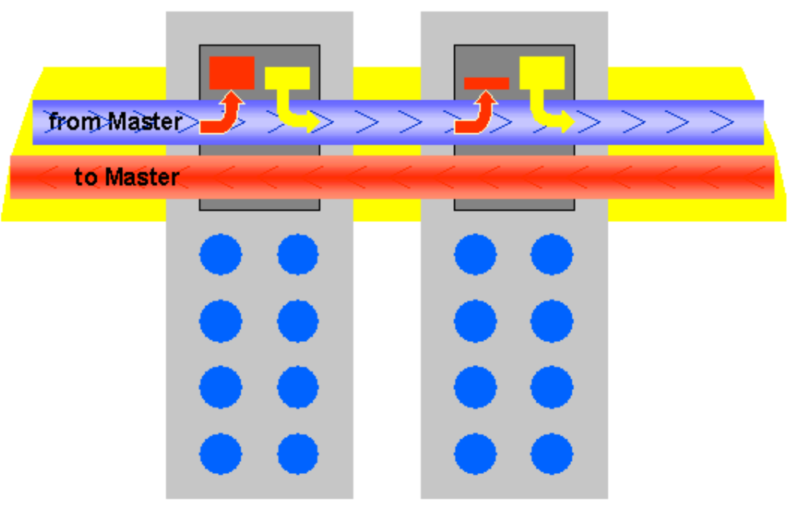
\includegraphics[width=0.7\linewidth]{./images/EtherCAT.png}
		\caption{Telegrammbearbeitung \cite{ethercat}}
		\label{fig:EtherCAT}
	\end{figure}\\
	Dabei wird auf dem gesamten Bus vom Ethernet-Protokoll nach IEEE 802.3 nicht abgewichen. Bit-Fehler werden so durch die CRC-Prüfsumme erkannt. Neben der Stern-Topologie unterstützt EtherCAT auch eine Linien- oder Baum-Struktur und viele weitere.
	EtherCAT zeichnet sich durch geringe Laufzeitverzögerungen und eine hohe Datenrate aus. Beispielsweise können 1000 E/as in nur 30 \(\mu s\) aktualisiert werden und auch eine Übertragungsrate GBit-Bereich ist mit Erweiterung möglich. \cite{ethercat}\\
	\label{subsec:EthernetFeldbus}
	Multi-Master Bussen (z.B. CAN oder TCP/IP) vs. Mono-Master
	
	\section{TCP/IP}
	TCP/IP (Transmission Control Protocol/Internet Protocol) ist das meist verwendete Netzwerkprotokoll weltweit und zudem frei zugänglich. Durch dieses Protokoll wird definiert, wie Daten durch Netzwerkkommunikationshardware versendet und empfangen werden kann. Welches Übertragungsmedium verwendet wird ist  nicht definiert, sodass sich neben LAN z.B. auch WLAN einsetzen lässt.\cite{CS9_TCP} \cite{kim2016service} \\
	TCP/IP ist nicht echtzeitfähig, stellt jedoch eine gute Ergänzung zu den Echtzeitprotokollen dar, um nicht zeitkritische Daten, wie z.B. zur Diagnose oder  Visualisierung zu übertragen. Bei TCP/IP handelt es sich um eine sichere Datenübertragung die Nachrichten in einen Bytestrom verpackt und entpackt. Vom Sender zum Empfänger durchlaufen die Daten vier Schichten (vgl. Abbildung \ref{fig:Schichtenmodell}). Für eine sichere fehlerfreie Übertragung werden die eigentlichen Daten ergänzt um die MAC-/IP- und TCP-Header. Das CRC-Feld stellt eine Art Prüfsumme, mit welcher die Korrektheit der übertragenen Daten überprüft wird. \cite{hering2012elektrotechnik}
	\begin{figure}[!ht]
		\centering
		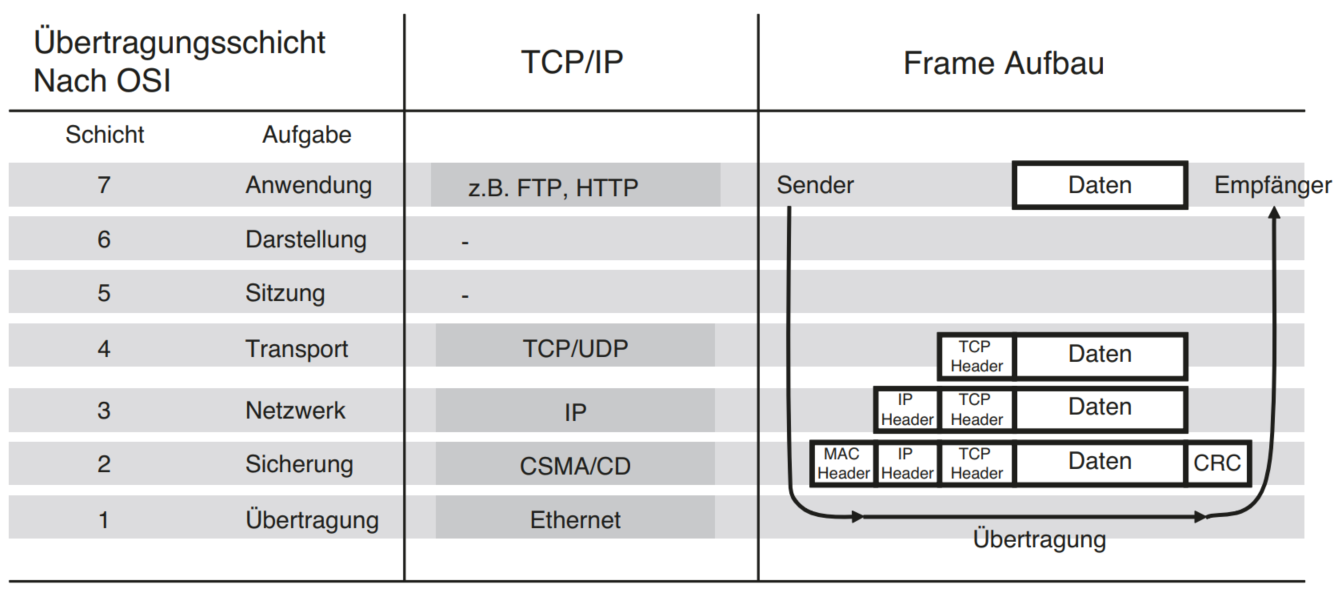
\includegraphics[width=1.0\linewidth]{./images/Schichtenmodell_TCP_IP.png}
		\caption{Schichtenmodell TCP/IP \cite{hering2012elektrotechnik}}
		\label{fig:Schichtenmodell}
	\end{figure} \\
	TCP/IP setzt sich aus den Protokollen TCP und IP zusammen.\\
	\\
	\textbf{TCP}\\
	Das Ziel von TCP ist eine fehlerfreie Datenübertragung. Hierzu muss der Empfänger die korrekt erhaltenen Daten, über eine Nachricht, die an den Sender zugesendet wird, bestätigen. Die Überprüfung der Korrektheit erfolgt mit dem CRC-Segment. Erhält dieser Sender diese Bestätigung nicht wird erneut versucht die Daten zu versenden. Hierdurch ist eine fehlerfreie und lückenlose Datenübertragung, selbst bei Netzwerkproblemen garantiert, was jedoch die Prozesse verlangsamt. Eine Alternative zu TCP ist UDP (User Datagram Protocol) . Hierbei erhält der Absender keine Bestätigung, dass die Daten korrekt empfangen wurde. Der Sender fährt direkt mit der Versendung der nächsten Pakete durch. Eine fehlerfreie Übertragung ist nicht garantiert, jedoch ist sie im Vergleich zu TCP schneller. Sowohl TCP, als auch UDP bauen auf dem Internetprotokoll IP auf. \cite{CS9_TCP}\\
	\\
	\textbf{IP} \\
	Das IP-Protokoll arbeitet auf der Internet bzw. IP-Schicht des TCP/IP-Protokolls, was der Netzwerkschicht des OSI-Modells entspricht. Die Ausgabe des IP-Protokolls ist es Datenpakete vom Sender zum Empfänger zu übertragen. Eine Datenüberprüfung und Fehlerkorrektur erfolgt nicht, sodass Daten verloren gehen können oder fehlerbehaftet sind. Die Garantie für die korrekte Datenlieferung geschieht durch das TCP-Protokoll. Das IP-Protokoll verwendet IP-Adressen, um Netzwerkknoten zu identifizieren. Mit Hilfe derer Adressen wird die Nachricht durch das Netz geroutet. Es wird ein idealer Weg zwischen Sender und Empfänger gesucht. \cite{harnisch2009netzwerktechnik} \cite{riggert2002rechnernetze} Es gibt zwei Versionen des IP-Protokolls IPv4 und IPv6. Bei IPv4 besteht die IP-Adresse aus 32 Bit, bei IPv6 aus 128 Bit, was die Anzahl der eindeutigen Adressen erhöht. Aufgrund der zunehmenden Geräteanzahl wird in der Zukunft IPv6 der Standard werden. Heute dominiert jedoch IPv4. \cite{riggert2002rechnernetze} \\
	Eine MAC-Adresse (Medium Access Control) ermöglicht eine eindeutige Identifikation eines Gerätes im Netzwerk. Da allerdings meist herstellerübergreifende Netzwerke eingesetzt werden, ist die IP-Adresse für eine eindeutige Identifikation besser geeignet. Diese kann entweder manuell oder automatisch zugewiesen werden. Der Aufbau einer IP-Adresse nach IPv4 ist nachfolgend dargestellt (vgl. Abbildung \ref{fig:IP-Adresse}).  \cite{hering2012elektrotechnik}
   	\begin{figure}[!ht]
   		\centering
   		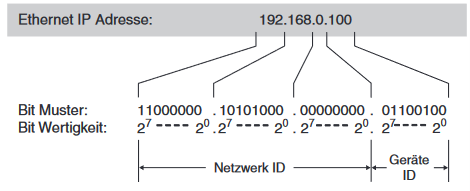
\includegraphics[width=0.70\linewidth]{./images/IP Adresse Aufbau.png}
   		\caption{IP-Adresse Aufbau \cite{hering2012elektrotechnik}} 
   		\label{fig:IP-Adresse}
   	\end{figure}
   	\\
   	\\
   	\textbf{Netzwerkarchitektur}\\
   	Während Netzwerke in ihrer Topologie, wie z.B. Bus, oder Stern-Topologie unterschieden werden können, kann auch eine Aufteilung nach Architekturtyp erfolgen. Neben der monolithischen Architektur und der Client-Server-Architektur gibt es Cloud-, Edge- und Fog-Computing. In der monolithischen Architektur existiert nur ein zentraler Rechner. An diesen werden externe Geräte angebunden, die selbst keine Rechenleistung aufweisen. Bei Cloud-, Edge- und Fog-Computing wird ein Teil der Netzwerktechnik an externe Organisationen ausgelagert. Eine externe Organisation kann ein Provider sein, der ein Server bereitstellt. \\
   	Im nachfolgenden soll die Client-Server-Architektur näher erläutert werden, da diese von Relevanz für diese Arbeit ist.
   	Bei der Client-Server-Architektur stellt der Client Anfragen an den Server, welche dieser beantwortet. Dieser Ablauf ist als Sequenzdiagramm in Abbildung \ref{fig:Sequenz Server-Client} dargestellt.\\
   	\begin{figure}[!ht]
   		\centering
   		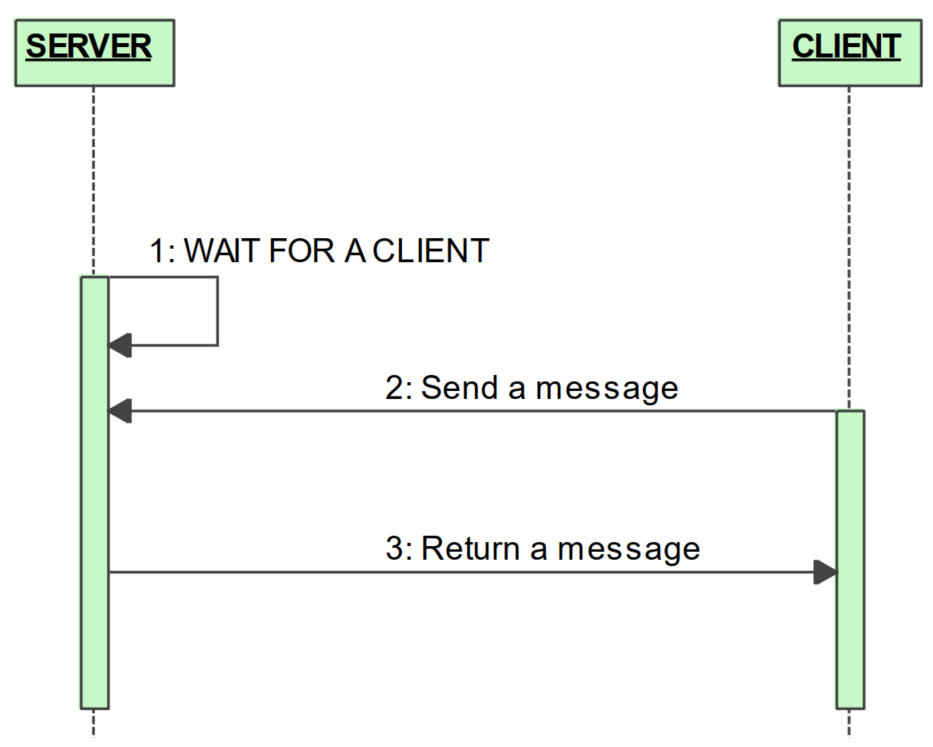
\includegraphics[width=0.50\linewidth]{./images/Sequenzdiagramm_Server_Client.png}
   		\caption{Sequenzdiagramm Server-Client-Architektur \cite{CS9_TCP}} 
   		\label{fig:Sequenz Server-Client}
   	\end{figure} \\   	
   	Charakteristisch für den Server ist dessen vergleichsweise hohe Rechenleistung, was es ermöglicht, dass mehrere Clients zeitgleich auf den Server zugreifen können. Veranschaulichen lässt sich dieses Prinzip mit dem Webbrowser, wie beispielsweise Google Chrome auf dem privaten Rechner. Dieser stellt den Client dar, welcher Anfragen an einen Webserver stellt, um aktuelle Daten passend zu seiner Anfrage zu erhalten. Auf dem Webserver wird beispielsweise ein Online-Shop verwaltet und mehrere Clients können zeitgleich auf diesen zugreifen. Das oben erwähnte Cloud-Computing basiert auf der Client-Server-Architektur, wurde jedoch nutzerfreundlicher gestaltet. \cite{IT-Sicherheit}
   	\label{sec:TCP/IP}
   	
   	\section{OPC/UA}
   	OPC UA (Open Platform Communication Unified Architecture) ist ein Protokoll zur Maschine-zu-Maschine-Kommunikation, aber auch zur Kommunikation zwischen SPS oder HMI (Human Interface) und Maschine. Es handelt sich hierbei um einen offenen und plattformunabhängigen Standard, welcher von der Open Platform Foundation (OPC) verwaltet wird. OPC UA basiert analog zu TCP/IP auf Ethernet und Internet. Es ist ebenso nicht echtzeitfähig. Das Kommunikationsprotokolls OPC UA ermöglicht eine vertikale und horizontale Kommunikation, da es die einzelnen Automatisierungsebenen verbindet. Somit kann von einem Roboter bis hin zur gesamten Fabriksteuerung alles verbunden werden, was OPC UA beliebt, um die Fabrik "Industrie 4.0" fähig zu machen. \cite{industrie40} \\
   	OPC UA basiert auf der Server-Client Architektur. Der OPC UA Server kann dann beispielsweise auf der SPS oder dem HMI (Human Interface) laufen und ein Roboter kann als OPC UA Client angebunden werden. Die Daten werden standardisiert und maschinenlesbar semantisch beschrieben, sodass herstellerübergreifende Kommunikation problemlos möglich ist. Sensordaten einer Maschine können dadurch an die Anlagensteuerung übertragen und visualisiert werden. OPC UA liefert dabei viele Vorteile: \cite{OPCUA}
   	\begin{itemize}
   		\item \textbf{Sicher:} IT-Sicherheit wurde bei der Entwicklung von OPC UA direkt mit eingeplant. Die Kommunikation und der Transport ist sicher und kann über Zugriffsrechte gesteuert werden.
   		\item \textbf{Plattformunabhängig:} Neben der Herstellerunabhängigkeit ist OPC UA unbhängig von der Programmiersprache, was es ermöglicht verschiedene Anlagen einfach zu verknüpfen.
   		\item \textbf{Einfach:} OPC UA ist auf Nutzerfreundlichkeit ausgelegt und das Festlegen von Kommunikationsprotokollen und der Aufbau von Nachrichten entfällt, sodass auch ohne Programmierkenntnisse eine Umsetzung möglich ist. 
   		\item \textbf{Big Data:} OPC UA ermöglicht einfaches Sammeln von Daten aus diversen Maschinen und von unterschiedlichsten Automatisierungsebenen. Hierdurch können sich umfangreiche Potentiale durch die Analyse der Daten ergeben und neue Geschäftsmodelle erschlossen werden. \\
   	\end{itemize}
   	Aufgrund dieser unterschiedlichsten Vorteile, wird OPC UA immer mehr im Bereich IoT und Industrie 4.0 eingesetzt. \cite{OPCUA}  \cite{industrie40}
   	
   	
   	\section{Stäubli-Roboter}
   	Stäubli ist ein in der Schweiz ansässiges Industrieunternehmen, welches in den Bereichen "Elektrische Verbindungen", "Fluidische Verbindungen","Textil" und "Robotik" tätig ist. Das Produktportfolio im Bereich Robotik umfasst Vier- und Sechsachs-Roboter, sowie kollaborative und mobile Roboter. \cite{StaubliUberUns}\\ Stäubli-Roboter sind nach IP 65 und IP 67 Staub- und Wasser- geschützt, wenn ein Arm mit Überdruckeinheit zum Einsatz kommt. Dies ermöglicht eine gründliche Reinigung aus Hygienezwecken und verhindert das Ansammeln von Staub im Roboter. Beispielsweise ist auch eine Reinigung mit Desinfektionsmittel oder Isopropylalkohol möglich. Zudem können die Roboter mit einem Lebensmittelverträglichem Öl eingesetzt werden. Stäubli-Roboter eignen sich daher insbesondere für Anwendungen in der Lebensmittel-, Pharma- und Medizin-Technik, in der viele andere Roboter die Hygieneanforderungen nicht erfüllen können. \cite{StaubliProduktubersicht}\\
   	\textbf{Roboter TX2 - 90}\\
   	Im Rahmen dieser Arbeit kommt der 6 Achs-Roboter TX2-90 zum Einsatz (vgl. Abbildung \ref{fig:TX90}). Dieser weist eine Tragkraft von 12 kg und eine Reichweite von 1000 mm auf. Die Wiederholgenauigkeit beträgt 0,03 mm und die maximale kartesische Geschwindigkeit 10,9 m/s. Der Roboter wiegt 114 kg und wird von der Robotersteuerung CS9 mit 2kVA gesteuert. Der Roboter ist für verschiedene, teils auch aggressive Reinigungsmittel geeignet, was für die Lebensmittelindustrie wichtig ist. Die Achsen können maximale Drehmomente zwischen 11 Nm (Achse 6) und 318 Nm (Achse 1) aufbringen.\\
   	Der Vorderarm des Roboters ist mit vier Magnetventilausgängen, von zwei 5/2-Wege-Magnetventilen versehen. Dies ermöglicht beispielsweise das Öffnen und Schließen eines Greifers.\\
   	Für den Roboter liegt ein Wartungsplan vor, welcher Wartungsarbeiten in unterschiedlichen Intervallen von monatlich bis 5-jährig vorsieht. Diese reichen von einfachen Sichtprüfungen und Bremstests über Ölwechsel und Dichtungstausch bis hin zum Auswechseln von Achsen. \cite{X90}
   	\begin{figure}[!ht]
   		\centering
   		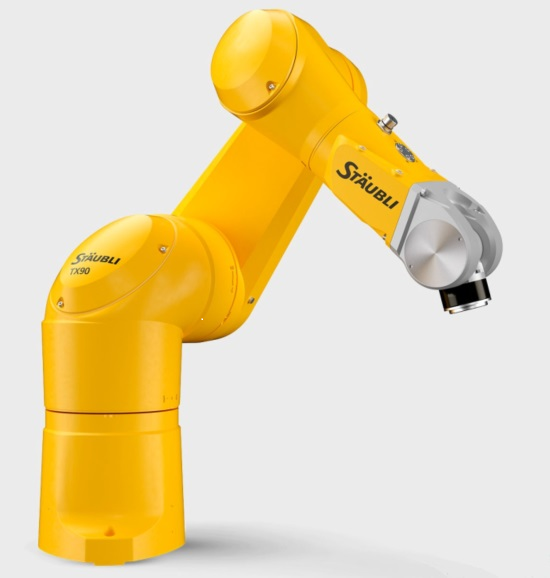
\includegraphics[width=0.50\linewidth]{./images/X90.png}
   		\caption{Stäubli TX2 - 90 \cite{X90}} 
   		\label{fig:TX90}
   	\end{figure}
   	\\
   	\subsection{Controller CS9}
   	Der CS9 Controller übernimmt die Steuerung und Versorgung des TX2 - 90 (vgl. Abbildung \ref{fig:CS9}).
   	\begin{figure}[!ht]
   		\centering
   		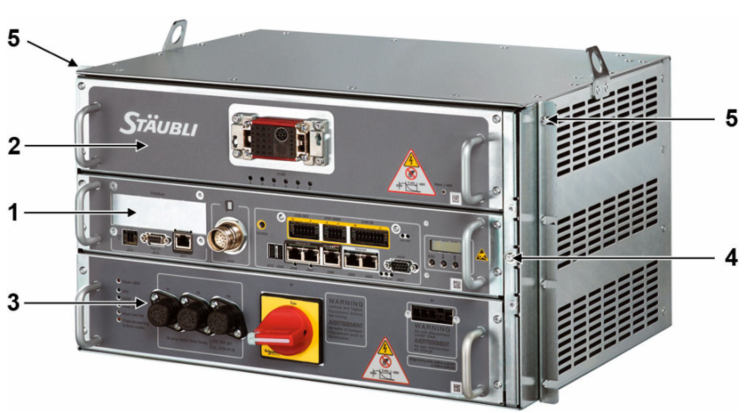
\includegraphics[width=0.70\linewidth]{./images/CS9.png}
   		\caption{Stäubli CS9 Controller \cite{CS9}} 
   		\label{fig:CS9}
   	\end{figure}
   	Der Computer-Einschub (1) beeinhaltet Karten, für die Sicherheitssteuerung, Bewegungssteuerung und die externe Kommunikation. Der Verstärker-Einschub (2) wandelt mit Hilfe von digitalen Achsverstärkern Bewegungsvorgaben in Motorströme um. Er beinhaltet zudem die Schnittstelle, an dem der Roboter angeschlossen wird. Der Stromversorgungs-Einschub (3) wandelt die Netzversorgungsspannung für die zuvor genannten Einschübe um und versorgt diese. Zudem existiert ein Anschluss für eine Antistatikmanschette (4), sowie Befestigungsmöglichkeiten (5).
   	\begin{figure}[!ht]
   		\centering
   		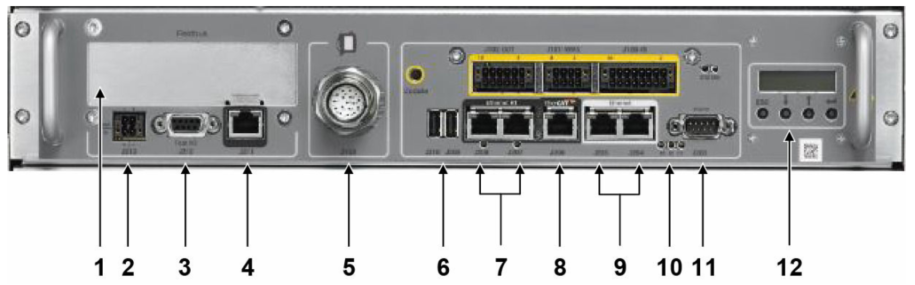
\includegraphics[width=0.70\linewidth]{./images/ComputerEinschub.png}
   		\caption{CS9 Controller Computer-Einschub \cite{CS9}} 
   		\label{fig:ComputerEinschub}
   	\end{figure}
   	Der Computer-Einschub (vgl. Abbildung \ref{fig:ComputerEinschub}) besitzt eine Vielzahl an Kommunikationsschnittstellen, die in der Tabelle nachfolgend dargestellt sind (vgl. Tabelle \ref{table:ComputerEinschub}).
   	\begin{longtable}{|p{1cm}|p{12cm}|}
   		\caption{CS9 Controller Computer-Einschub}
   		\label{table:ComputerEinschub}\\
   		\hline
   		Nr. & Bezeichnung  \\ [0.5ex] 
   		\hline
   		\endhead
   		1 & Feldbus, Option für PCIe-Karte  \\ 
   		2 & Anschluss für optionale externe 24 V Stromversorgung  \\
   		3 & Schnelle Ein-/Ausgänge  \\
   		4 & EtherCAT Port (Reserviert) \\
   		5 & Anschluss Handbediengerät  \\
   		6 & USB-Ports \\  
   		7 & Echtzeit-Ethernet-Slave (EtherCAT, Sercos III, EtherNet/IP, PROFINET  \\ 
   		8 & EtherCAT-Master  \\ 
   		9 & Ethernet-Ports (1000 MBits/s und 100 MBits/s)  \\
   		10 & Status LEDs  \\ 
   		11 & serielle Verbindung RS232  \\
   		12 & Benutzerschnittstelle  \\  
   		\hline
   	\end{longtable}
   	 An den CS9 Controller kann kann ein Handbediengerät angeschlossen werden (5), was z.B.  manuelles Verfahren oder einfachere Programmier- und Konfigurationsarbeiten ermöglicht. Hervorzuheben ist zudem der Echtzeit-Ethernet-Slave-Anschluss (7), durch welchen die Steuerung z.B. über EtherCAT mit einer SPS verbunden werden kann. Zusätzlich steht ein EtherCAT-Master-Anschluss (8) zur Verfügung. Die CS9 ermöglicht es somit den Roboter als EtherCAT-Slave oder als EtherCAT-Master zu betreiben.\\
   	 Zudem stehen zwei Ethernet-Ports (9) zur Verfügung, was eine externe Kommunikation z.B. über TCP/IP ermöglicht. Die IP-Adresse der Ethernet-Ports kann frei konfiguriert oder automatisch vergeben werden. Als Dateiübertragungs-Serverprotokoll dient "FTPS+FTP". FTP wird als Standardeinstellung verwendet, während FTPS eine sichere Authentifizierung ermöglicht. \\
   	 Auf der CS9-Steuerung lassen sich sogenannte Sockets konfigurieren, welche eine TCP/IP oder eine UDP/IP - Kommunikation ermöglichen. Die Konfiguration kann dabei im Client oder Server-Modus erfolgen. \cite{CS9}
   	 
   	\subsection{Programmiersprache VAL3}
   	Die Programmierung des Roboters kann auf dem Handbediengerät erfolgen oder bevorzugt in der Stäubli Robotic Suite (SRS). In der SRS kann neben der Programmierung eine Simulation des Roboters inklusive 3D-Darstellung erfolgen, sodass die Programme direkt getestet werden können.\\
   	"VAL 3" ist eine höhere Programmiersprache und besitzt spezielle Steuerungsfunktionen für den Roboter zur Bewegungsteuerung und zur Ansteuerung von Ein-/Ausgängen. \cite{VAL3}\\
   	\textbf{Programm} \\
   	In einer Applikation können mehrere Programme angelegt werden. Diese verhalten sich wie Funktionen und lassen sich aufrufen. Zur Ausführung der VAL3-Applikation wird standardmäßig das Prgoramm "start()" gestartet, welches vergleichbar mit einer "main-Funktion" ist. Von hier lassen sich wiederum andere Programme aufrufen. Bei Beendigung der Applikation wird das Programm "stop()" einmalig aufgerufen, um z.B. von dort Tasks zu beenden.\\
   	Programme lassen sich auch als Task ausführen. Bei einer Task handelt es sich um ein Programm welches zu einem gewissen Zeitpunkt ausgeführt wird. Üblicherweise wird beispielsweise die Bewegungssteuerung und die Kommunikation in eigene Tasks ausgelagert. Es wird ein möglichst gleichzeitiges Ausführen der Tasks angestrebt. Da die Steuerung jedoch nur einen Prozess besitzt, ist es jedoch nur möglich eine Task auszuführen. Die augenscheinliche Parallität, wird dadurch erreicht, dass die Tasks sequentiell sehr schnell hintereinander ausgeführt werden. Dabei wird nicht die gesamte Task abgearbeitet, sondern einige wenige Anweisungen. Eine Task erhält zudem eine Priorität, die angibt, wie viele Programmzeilen ausgeführt werden bis die nächste Task abgearbeitet wird. Eine hohe Priorität sorgt daher für ein schnellstmögliches Abarbeiten dieser Task. Wird in einer Task eine Wartezeit ("delay") ausgeführt, pausiert diese Task und der Prozessor arbeitet nur die anderen Tasks ab. Neben den erwähnten asynchronen Tasks bietet VAL 3 ebenso synchrone Tasks.
   	\begin{figure}[!ht]
   		\centering
   		\includegraphics[width=0.80\linewidth]{./images/tasks.png}
   		\caption{Sequentielle Anordnung von Tasks \cite{VAL3}} 
   		\label{fig:TX90}
   	\end{figure} \\
   	\textbf{Datentypen}\\
   	In VAL 3 gibt es verschiedene einfache Datentypen, die nachfolgend kurz erläutertet werden. Neben den einfachen Datentypen gibt es weitere Datentypen, die z.B. Punkte für die Bewegungsteuerung darstellen. Auf eine Erläuterung dieser wird verzichtet, da diese Kommunikation nicht benötigt werden.
   	\begin{itemize}
   		\item \textbf{BOOL:} Variablen und Konstanten von diesem Typ können true und false annehmen.
   		\item \textbf{NUM:} Datentyp zur Darstellung von numerischen Werten mit 14 signifikanten Stellen. Im Gegensatz zu vielen gängien Programmiersprachen wird in VAL 3 nicht zwischen verschiedenen Zahlenformaten unterschieden. Dieser Datentyp kann von ganzzahligen Werten bis hin zu Kommazahlen alles abbilden.
   		\item \textbf{BITFELD:} Dieser Datentyp ermöglicht es eine Bitfolge z.B. von booleschen Werten oder digitalen Ein- und Ausgängen kompakt abzuspeichern.
   		\item \textbf{STRING:} In Variablen und Konstanten diesen Typs können Zeichenketten mit einer Länge von bis zu 256 Byte gespeichert werden. Die interne Zeichencodierung erfolgt mit Unicode UTF 8. Bei ASCII-Zeichen entspricht die Läge von 256 Bytes somit 234 Zeichen. Initialisiert werden Variablen diesen Datentyps standardmäßig mit einem leeren String ("").
   		\item \textbf{DIO:} Dieser Datentyp ermöglicht es aus dem Programm auf die digitalen Ein-/Ausgänge der Steuerung zuzugreifen. Hierzu speichert die dio-Variable einen Link zu der entsprechenden Hardware in Form einer physischen Adresse.
   		\item \textbf{AIO:} Mit Hilfe diesen Datentyps können die analogen Ein- und Ausgänge der Steuerung verknüpft werden.
   		\item \textbf{SIO:} Dieser Datentyp ermöglicht es einen seriellen Port oder einen Ethernet Socket Anschluss zu verknüpfen. Dadurch kann beispielsweise eine TCP/IP - Nachricht geschrieben oder gelesen werden, in dem der Variable des Datentyps ein Wert zugewiesen wird oder ein Wert abgelesen wird. \\
   	\end{itemize}
   	\textbf{Robotersteuerung}\\
   	Neben Funktionalitäten die klassische Programmiersprachen aufweisen, benötigt VAL 3 insbesondere Möglichkeiten, um den Roboterarm zu steuern. Exemplarisch werden einige Befehle kurz vorgestellt. Zum Einsatz
   	\begin{itemize}
   		\item \textbf{disable / enable Power:} Hiermit lässt sich die Armleistung ab bzw. einschalten. Für den lokalen, manuellen oder Testbetrieb hat diese Funktion keinen Einfluss.
   		\item \textbf{getVersion:} Mit dieser Anweisung lassen sich die Version der Hardware- und Software - Komponenten des Robotercontrollers abfragen.
   		\item \textbf{movej:} Dieser Befehl führt eine Bewegung zu einem Punkt aus. Angegeben werden muss die Winkelposition der Achsen für den Zielpunkt (vom Datentyp "joint"), die Geometrie des Werkzeuges (Datentyp "tool") und Bewegungsdaten, wie Geschwindigkeit und Beschleunigung (Datentyp "msdec").
   		\item \textbf{movel:} Dieser Befehl ermöglicht im Gegensatz zum Vorangegangen eine lineare Bewegung. Anstelle der Winkelpositionen als Ziel wird eine kartesische Zielkoordinate (Datentyp "point") vorgegeben.  \\
   	\end{itemize}
   	\section{Anlagensteuerung}
   	Ein Roboter ist meist nur ein Teil einer Automatisierungslösung. Dieser kann um Förderbänder, Sensoren und andere Aktoren ergänzt werden. Wie die Steuerung dieser Gesamtanlage umgesetzt wird unterscheidet sich von Anlagenautomatisierer zu Anlagenautomatisierer. Hier soll die bei robomotion gängige Umsetzung aufgezeigt werden, da diese relevant für das Gesamtverständnis und die Konzeptionierung der Komponenten ist. \\
   	\textbf{SPS}\\
   	Zentrales Element jeder Anlagenautomatisierung ist eine Beckhoff-SPS, welche auf einem IPC läuft. Diese ist für die Ablauflogik und "Intelligenz" der Anlage zuständig. Auf anderen Bestandteilen, wie z.B. in einer Robotersteuerung ist hingegen nur eine geringe Komplexität abgebildet. In der Robotersteuerung werden meistens Kommandos mit Jobnummern angelegt, wie beispielsweise die Bewegung von Punkt A zu Punkt B. Durch den Aufruf der Jobnummer durch die SPS erhält der Roboter den Befehl zur Bewegungsausführung und meldet eine erfolgreich durchgeführte Bewegung der SPS zurück. Welche Bewegungen in welcher Reihenfolge und wann durchgeführt werden, ist dementsprechend nicht in der Robotersteuerung, sondern in der SPS-Steuerung programmiert.\\
   	\textbf{roboTools} \\
   	Weiterer Bestandteil der Automatisierung ist ein Programm namens "roboTools", welches zur Anlagenvisualisierung dient. Dieses läuft auf einem Windows-Betriebssystem in Form einer WPF (Windows Presentation Foundation), des ".NET"-Frameworks. Das Programm roboTools mit seiner grafischen Oberfläche enthält verschiedene Diagnosewerkzeuge und kann dem Anlagenbediener Informationen über bspw. Störungen oder der Anlagenauslastung ausgeben und visualisieren. Die Daten hierfür bezieht roboTools überwiegend von der SPS. \\
   	\textbf{roboVision}\\
   	Häufig werden in Anlagen Industriekameras eingesetzt, um die Position von Objekten zu ermitteln oder eine automatisierte Qualitätskontrolle vorzunehmen. Zur Weiterverarbeitung der Kameradaten, um die Position oder die Qualitätsgüte zu bestimmen kommt das Programm "roboVision" zum Einsatz. Wie roboTools handelt es sich um ein WPF-Anwendung, welche auf einem Windows-Betriebssystem läuft. \\
   	\textbf{Hardware und Zusammenspiel}\\
   	Sowohl roboTools, als auch roboVision laufen auf einem IPC. Dies kann der selbe IPC sein, auf dem bereits die SPS läuft. Insbesondere für roboVision wird jedoch meist ein eigenständiger leistungsfähiger IPC eingesetzt, da für die Bildverarbeitung eine hohe Rechenleistung zur Verfügung stehen muss. Für die Umsetzung der Kommunikationsschnittstelle, spielt dies jedoch keine große Rolle, da sich alle IPCs in einem Netzwerk befinden. Da es sich um getrennte Programme handelt können diese alle als eigenständige Einheiten behandelt werden, auch wenn sie auf dem selben IPC laufen. Das Zusammenspiel dieser Komponenten ist nachfolgend dargestellt (vgl. Abbildung \ref{fig:Anlagensteuerung}).\\
   	
   	\begin{figure}
   		\centering
   		\begin{tikzpicture}[node distance=2cm]
   			
   			% Erste Reihe von Boxen
   			\node[draw, rectangle] (box1) at (-2cm,0) {Beckhoff-SPS};
   			\node[draw, rectangle] (box2) at (2cm,0) {roboTools};
   			\node[draw, rectangle] (box3) at (6cm,0) {roboVision};
   			
   			% Zweite Reihe von Boxen
   			\node[draw, rectangle] (box4) at (-2,-2cm) {Roboter-Steuerung};
   			\node[draw, rectangle] (box5) at (6cm,-2cm) {Kamera};
   			
   			% Linien verbinden die Boxen
   			\draw (box1) -- (box2);
   			\draw (box2) -- (box3);
   			\draw (box1) -- (box4);
   			% \draw (box2) -- (box4);
   			\draw (box3) -- (box5);
   			
   		\end{tikzpicture}
   		\caption{Anlagensteuerung Aufbau}
   		\label{fig:Anlagensteuerung}
   	\end{figure}
   	
   	
   	
   	\section{WPF}
   	Da bereits roboTools und roboVision auf WPF beruhen, ist WPF von großer Relevanz für diese Arbeit. WPF basiert auf dem .NET - Framework.
   	Das .NET Framework ist eine Plattform für unterschiedliche Programmiersprachen, wie C\# oder Visual Basic  mit denen verschiedene Applikationstypen, wie Desktop, Web oder Mobile entwickelt werden können.\\
   	Das .NET-Framework ist eine Entwicklung von Microsoft. Die meisten Anwendungen können jedoch plattformübergreifend eingesetzt werden. Lediglich Desktopanwendungen, wie z.B. WPF sind an Windows gebunden.\\
   	\textbf{C\#}
   	Das .NET-Framework ist offen für verschiedenste Programmiersprachen, jedoch ist die Verwendung von C\# am geläufigsten und kommt in den vorhandenen Anwendungen von robomotion zum Einsatz. C\# ist eine Entwicklung speziell für .NET und kombinierte Konzepte und Bestandteile von Java, JavaSrcipt, C++ und Visual Basic. Dabei handelt es sich um eine vollwertige objektorientierte Sprache mit Eigenschaften, wie Vererbung und Kapselung.\\
   	\textbf{Programmierumgebung}\\
   	Visual Studio und DevOps\\
   	\textbf{WPF}
   
   	
   	\section{Bewertung}
   	In der Literatur wird meist das TCP Protokoll zur Datenübertragung eingesetzt, um die Korrektheit der Daten sicherzustellen. In \cite{groza2008using} kommt das Protokoll UDP zur Übertragung von Live-Kamera-Bildern zum Einsatz, da hier die Schnelligkeit über die Korrektheit zu stellen ist. Während in der Literatur z.B. in \cite{groza2008using} VPN zur IT-Sicherheit eingesetzt wird, kann dies im Rahmen des Projektes entfallen.
   	
	\newpage
	
	\chapter{Anforderungsdefinition}
	Die Aufgabenstellung und die grobe Anforderungsformulierung soll in diesem Kapitel mit Hilfe eines Lastenheftes in eine strukturierte Form gebracht werden. Das Lastenheft beschreibt, welche Funktionalitäten das zu entwerfende System aufweisen soll. Darüber hinaus kann das Lastenheft Rahmenbedingungen enthalten, wie z.B. zulässige Reaktionszeiten oder weitere Einschränkungen. Das Lastenheft wird in aller Regel vom Auftraggeber erstellt. Der Auftragnehmer beschreibt im Pflichtenheft durch welche Systemfunktionalitäten die Aufgaben erfüllt werden sollen und wie die Umsetzung technisch erfolgt. Das Lasten- und Pflichtenheft dient auch zur rechtlichen Absicherung der Vertragsparteien. Obwohl ein Lasten- und Pflichtenheft oft als Vertragsgrundlage entworfen wird und dies im Rahmen des Projektes nicht notwendig ist, soll ein Lastenheft eingesetzt werden. Dies ermöglicht es alle Anforderungen und Rahmenbedingungen zu berücksichtigen und diese im gesamten Projektverlauf im Blick zu behalten. Auf ein Pflichtenheft wird hingegen verzichtet. \cite{SoftwaretechnikBroy}
	Das Lastenheft wird in Muss- und Kann-Kriterien unterteilt. Während bei den Muss-Kriterien eine Erfüllung essentiell ist, stellen die Kann-Kriterien eine optionale Erweiterung dar, die dem System jedoch einen Mehrwert verschaffen.\\
	\begin{longtable}{|p{1cm}|p{10cm}|p{2cm}|}
		\caption{Lastenheft}
		\label{table:Lastenheft}\\
		\hline
		Nr. & Anforderung & Kann (K) / Muss (M) \\ [0.5ex] 
		\hline
		\endhead
		1 & Übertragung von Fehlermeldungen des Stäubli-Roboters an die Anlagenvisualisierung & M  \\ 
		2 & Übertragung von beliebigen Daten des Stäubli-Roboters an die Anlagenvisualisierung & M  \\
		3 & Übertragung von Daten z.B. Kameradaten von der Anlage an den Stäubli-Roboter & M  \\
		4 & Ausgabe der Roboterfehler auf der Anlagenvisualisierung in verständlicher Form (ausformuliert, Fehlercode genügt nicht) & M  \\
		5 & Funktionierende Feldbusverbindung zwischen Stäubli-Roboter und SPS & M  \\
		6 & Funktionierende TCP/Ip Kommunikation zwischen Stäubli-Roboter und Anlagenvisualisierung & M  \\  
		7 & Abspeichern der Fehler und der Daten in log-File & M  \\ 
		8 & Fehlerfreie und prozesssichere Kommunikation & M  \\ 
		\hline
		9 & Einsatz von mehreren Stäubli-Robotern zeitgleich soll möglich sein & K  \\
		10 & Vorgabe von der Anlagenvisualisierung, wie häufig Daten versendet werden sollen & K  \\ 
		11 & Visualierung der Daten & K  \\
		12 & Verwertung der Daten, um Warnungen oder ähnliches auszugeben & K  \\  
		\hline
	\end{longtable}
	Im Rahmen dieser Arbeit ist die Feldbus-Verbindung zwischen SPS und Roboter zu entwerfen. Der Fokus liegt jedoch auf der TCP/IP-Verbindung zwischen Roboter und Anlagenvisualisierung. Darüber hinaus ist das Programm für den Roboter zu konzeptionieren und zu implementieren. Das andere Ende der TCP/IP-Verbindung stellt die Anlagenvisualisierung dar. Dort sollen auch die Fehlermeldungen ausgegeben und die Daten visualisiert werden. Als Anlagenvisualisierung dient bei robomotion robotools. Die zu entwerfende WPF-Anwendung zur TCP/IP-Kommunikation und zur Datenvisualisierung kann nach Projektende in roboTools integriert werden. Dies soll jedoch nicht mehr Teil der Arbeit sein. Die zu entwerfende WPF-Anwendung wird im Rahmen dieser Arbeit vereinfacht als Anlagenvisualisierung bezeichnet. Die bestehende Anwendung roboVision erstellt auf Basis von Kamerabildern Positionsdaten von zugreifenden Objekten. Diese Positionsdaten können über die Beckhoff-spezifische Verbindung namens "ADS" zu roboTools und somit auch zur entwerfenden WPF-Anwendung übertragen werden. Die SPS ist mit roboTools ebenso über ADS verbunden, was für diese Arbeit jedoch keine Relevanz hat.  Eine Konzeptionierung und Implementierung des SPS-Programms kann entfallen, da die Kommunikation mit einer Feldbus-Verbindung in der Beckhoff-SPS bei robomotion Stand der Technik ist und dadurch aus anderen Projekten übernommen werden kann. Das Zusammenspiel all dieser Komponenten ist nachfolgend dargestellt, wobei die im Rahmen dieser Arbeit zu entwerfenden Komponenten farbig markiert sind (vgl. Abbildung \ref{fig:Anlagensteuerung_Aufgabe}).
	\begin{figure}
		\centering
		\begin{tikzpicture}[node distance=2cm]
			% Erste Reihe von Boxen
			\node[draw, rectangle, align=center] (box1) at (-3cm,0) {Beckhoff-SPS\\ };
			\node[draw, rectangle, align=center, fill=green!20] (box2) at (3cm,0) {Anlagenvisualisierung\\(roboTools)};
			\node[draw, rectangle, align=center] (box3) at (9cm,0) {Bildverarbeitung\\(roboVision)};
			
			% Zweite Reihe von Boxen
			\node[draw, rectangle, fill=green!20] (box4) at (0,-3cm) {Roboter-Steuerung};
			\node[draw, rectangle] (box5) at (9cm,-3cm) {Kamera};
			
			% Linien verbinden die Boxen und Beschriftungen hinzufügen
			\draw (box1) -- node[above] {ADS} (box2);
			\draw (box2) -- node[above] {ADS} (box3);
			\draw (box1) -- node[left, fill=green!20] {Feldbus} (box4);
			\draw (box2) -- node[right, fill=green!20] {TCP/IP} (box4);
			\draw (box3) -- node[right] {} (box5);
		\end{tikzpicture}
		\caption{Gesamtanlage zu entwerfende Komponenten}
		\label{fig:Anlagensteuerung_Aufgabe}
	\end{figure}

	\label{chap:Anforderungsdefinition}
	\chapter{Konzeptionierung}
	In diesem Kapitel soll das Gesamtsystem und seine Bestandteile konzeptioniert werden. Hierfür werden die Komponenten der Anlage benannt und ihre Funktionen grob skizziert. Dies erfolgt mit Hilfe eines UML-Klassendiagramms (vgl. Abbildung \ref{fig:UMLKlassenAnlage}) \cite{Sommerville}.
	!UML-Diagramm.	Anwendungsfälle definieren, Rahmenbedingungen identifizieren, Anforderungen aus Lastenheft verfeinern. Softwarekomponenten definieren und im Komponentendiagramm darstellen gemäß UML.!
	
	\begin{figure}
		 \begin{tikzpicture}
		 	\umlclass[x=0]{SPS}{
		 		- Eingänge : int \\
		 		- Ausgänge : bool \\
		 	}{
		 		+ sendeBefehle() : void \\
		 		+ empfangeBestätigungen() : void
		 	}
		 	
		 	\umlclass[x=8]{Anlagenvisualisierung}{
		 		- Betriebsmodus : string \\
		 		- Logger : string\\
		 		- Graphik: \\
		 		
		 	}{
		 		+ erfrageRoboterDaten() : void \\
		 		+ empfangeRoboterDaten() : void \\
		 		+ sendePositionen(): void\\
		 		+ visualisiereFehlermeldungen(): void\\
		 		+ visualisiereRoboterdaten(): void \\
		 		+ schreibtLogFile(): void
		 	}
		 	\umlclass[x=4, y=-8]{Roboter}{
		 		- Geschwindigkeit : float \\
		 		- Temperatur: int \\
		 		- Drehmoment: int \\
		 		- Fehlermeldung: string
		 	}{
		 		+ bewegen() : void \\
		 		+ empfangeBefehle() : void \\
		 		+ sendeBestätigungBewegungsausführung(): void\\
		 		+ sendeDaten(): void \\
		 		+ sendeFehlermeldungen(): void
		 	}
		 	% Verbindungslienie zwischen SPS und Roboter mit Multiplicitäten
		 	\umlassoc[arg=steuert,pos=0.5]{Roboter}{SPS}
		 	\umlassoc[arg=kommuniziert mit,pos=0.5]{SPS}{Anlagenvisualisierung}
		 	\umlassoc[arg=kommuniziert mit,pos=0.5]{Anlagenvisualisierung}{Roboter}
		 	\umlassoc{Roboter}{SPS}
		 \end{tikzpicture}
		 \caption{UML-Klassendiagramm Gesamte Anlage}
		 \label{fig:UMLKlassenAnlage}
	\end{figure}
	Das UML-Diagramm zeigt die Komponenten SPS, Roboter und Anlagenvisualisierung auf. Die Kommunikation zwischen SPS und Roboter erfolgt mittels Feldbus, zwischen Anlagenvisualisierung und Roboter mittels TCP/IP. Daher soll im ersten Schritt der Feldbus und die TCP/IP-Verbindung konzeptioniert werden. Erst anschließend kann das Programm des Roboters und der Anlagenvisualisierung konzeptioniert werden, da dieses maßgeblich abhängig von der Wahl und dem Aufbau der Kommunikationsverbindung ist. Nachdem die Feldbus-Verbindung und die TCP/IP-Verbindung konzeptioniert wurden sollen die zu übertragenden Daten für die TCP/IP-Verbindung konzeptioniert werden. Anschließend erfolgt die Konzeptionierung der Software für den Stäubli-Roboter und die Anlagenvisualisierung.
	 
	\section{Feldbus-Verbindung}
	Aufgabe der Feldbusverbindung ist die Kommunikation zwischen dem Stäubli-Roboter und der Beckhoff-SPS sicherzustellen. Hierzu werden einerseits Befehle, wie zur Bewegungsdurchführung zum Roboter übertragen, andererseits Informationen, wie z.B. eine Bestätigung der vollendeten Bewegung zurück an die SPS gesandt.\\
	\textbf{Wahl des Feldbusses}\\
	In Kapitel \ref{sec:Feldbus} wurden die Feldbusse in Standard-Feldbusse und Ethernet basierende Feldbusse unterteilt. Die Wahl fällt hierbei auf einen Ethernet-basierenden Feldbus, weil dies der aktuelle Stand der Technik darstellt und zudem firmenintern ausnahmslos eingesetzt wird. Nach Kapitel \ref{subsec:EthernetFeldbus} sind Profinet, Ethernet/IP, EtherCAT und Sercos III häufig eingesetzte Ethernet basierende Feldbusse. Eine Gegenüberstellung der Vor- und Nachteile der einzelnen Feldbusse und eine Auswahl anhand dieser Kriterien kann jedoch entfallen, da zwei Argumente für den Einsatz von EtherCAT, alle anderen Kriterien überwiegen.\\
	Zum Einsatz kommt eine Beckhoff-SPS. EtherCAT ist eine Entwicklung von Beckhoff und daher bestmöglichst auf die SPS von Beckhoff abgestimmt.\\
	Darüber hinaus, kommt unternehmensintern bereits in anderen Projekten EtherCAT zum Einsatz. Die Wahl von EtherCAT bringt daher folgende Vorteile mit sich
	\begin{itemize}
		\item \textbf{Know How: } Firmenintern hat sich durch den wiederholten Einsatz von EtherCAT bereits eine große Wissenbasis und Erfahrung aufgebaut. Bei schwerwiegenderen Problemen ermöglicht dies eine einfachere Fehlersuche.
		\item \textbf{Schulungszwecke: } Durch andere Projekte sind beispielsweise die Service-Techniker bereits in EtherCAT geschult. Die Buchung einer zeit- und kostenintensiven Schulung für einen anderen Feldbus kann entfallen
		\item \textbf{Standardisierung:} Der Einsatz von vielen unterschiedlichen Systemen erhöht den Aufwand in Dokumentation und Einkauf. Daher wird versucht die Varianz möglichst gering zu halten und auf einen Standard, welcher bereits eingesetzt und verbreitet ist zu setzen.\\
	\end{itemize}
	\textbf{Master-Master vs. Master-Slave}\\
	Standardmäßig wird jedoch sowohl die Beckhoff-SPS, als auch der Stäubli Roboter als Master eingesetzt. Jedoch ist EtherCAT rein für Master-Slave-Kommunikation ausgelegt, d.h. es kann nur ein Master existieren. \cite{ethercat}	Beckhoff bietet jedoch eine spezielle Bridge-Klemme (EL6692) an, die es erlaubt EtherCAT-Stränge zu synchronisieren und ein Datenaustausch zwischen den einzenen Strängen zu ermöglichen. Da jeder EtherCAT-Strang einen eigenen Master besitzt ermöglicht die Bridge den Einsatz von mehreren Mastern. \cite{Bridge} Hierdurch entstehen jedoch zusätzliche Kosten und auch die Komplexität des Systems steigt. Da sowohl die Stäubli-Steuerung, als auch die SPS ebenso als Slave konfiguriert werden kann, entfällt die Entscheidung auf die Master-Slave-Kommunikation, um die zusätzliche Master-Master-Klemme einzusparen.\\
	\textbf{Wahl des Masters} \\
	Nachdem die Entscheidung für eine Master-Slave-Architektur gefallen ist, muss festgelegt werden, ob die Beckhoff-SPS oder der Stäubli-Roboter als Master konfiguriert wird. Da der Einsatz von mehreren Stäubli-Robotern in Automatisierungslösungen denkbar ist, könnte nicht jeder Stäubli-Roboter als Master eingesetzt werden. Folglich wäre ein Stäubli-Roboter ein Master, die anderen Stäubli-Roboter, wie auch die SPS Slaves. Um diese Unterschiede in den einzelnen Stäubli-Robotern zu verhindern, ist es sinnvoll die Beckhoff-SPS als Master zu konfigurieren, sodass alle Stäubli-Roboter einheitlich als Slaves eingesetzt werden. Darüber hinaus ist die SPS der zentrale Teil der Anlagenautomatisierung, von welcher weitere Komponenten, wie Roboter anderer Hersteller gesteuert werden können, weshalb die Wahl der SPS als Master sinnvoll ist.\\
	Die Gesamtentscheidung zur Konfiguration ist nachfolgend mit Hilfe eines morphologischen Kastens dargestellt.\\
	
	\begin{NiceTabular}{@{}>{\bfseries}lcccc@{}}
		\CodeBefore [create-cell-nodes]
		\tikz \draw [red!50, line width=2pt, line join = round] 
		plot [samples at={3-2, 4-3, 5-2}] (\x) ;
		\Body
		\toprule
		\RowStyle[nb-rows=2]{\bfseries}  
		& \Block{1-4}{Konfiguration} \\ 
		\cmidrule{2-5}
		Parameters  & Option 1 & Option 2 & Option 3 & Option 4 \\ 
		\midrule
		Bussystem     & etherCAT      & Profinet  & Sercos III & Soft       \\
		Architektur & Master-Master       & Master-Slave  &   &      \\
		Master & SPS      & Stäubli           &       & \\ 
		\bottomrule
	\end{NiceTabular}
	
	
	\begin{tikzpicture}[
		font=\sffamily,
		circle mark/.style={
			draw=#1,
			shape=ellipse,
			thick,
			inner xsep=-3pt
		},
		circle mark finish/.style={
			circle mark=red
		},
		circle mark unfinish/.style={
			circle mark=green
		},
		line/.style={red, thick},
		line thick/.style={ultra thick}
		]
		\matrix [
		matrix of nodes,
		nodes={
			draw, 
			minimum width=2.6cm, 
			minimum height=.8cm, 
			anchor=center
		},
		row sep=-\pgflinewidth,
		column sep=-\pgflinewidth,
		nodes in empty cells,
		row 1/.style={nodes={draw=none}}
		] (m) {
			|[draw]| Merkmal &&&&\\
			Faktor 1 & etherCAT & profinet & Ethernet/IP & Sercos III \\
			Faktor 2 & Master-Master & Master-Slave & & \\
			Faktor 3 & SPS als Master & Stäubli als Master &  & \\
		};
		\node [draw, fit=(m-1-2)(m-1-5), inner sep=-.5\pgflinewidth, label=center:Ausprägung]{};
		
		\draw [line thick] 
		(m-1-1.north east) -- (m-4-1.south east)
		(m-1-1.south west) -- (m-1-5.south west)
		;
		
		\path [nodes=circle mark finish]
		(m-2-2) node (cm1) {\phantom{Ausprägung 1}}
		(m-4-4) node (cm3) {\phantom{Ausprägung 3}}
		;
		\path [nodes=circle mark unfinish]
		(m-3-3) node (cm2) {\phantom{Ausprägung 2}}
		;
		\draw [line] 
		(cm1.east) -- (cm2.west)
		(cm2.east) -- (cm3.west)
		;
	\end{tikzpicture}
	
	\section{TCP/IP-Verbindung}
	Nachdem die Feldbus-Verbindung konzeptioniert wurde, erfolgt die Auslegung der TCP/IP-Verbindung. Hierbei müssen viele Einzelentscheidungen getroffen werden, welche am Ende mit einem morphologischen Kasten zusammengefasst dargestellt werden.\\
	\textbf{Wahl der Architektur} \\
	Wie in Kapitel \ref{sec:TCP/IP} erläutert kommt für eine TCP/IP-Verbindung die Client-Server-Architektur zum Einsatz. Dabei kann entweder der Stäubli-Roboter oder die Anlagenvisualisierung als Server dienen. In der Literatur wird meist empfohlen, die Seite mit der höheren Rechenleistung als Server einzusetzen (vgl. Kapitel \ref{sec:TCP/IP}). Dies stellt in diesem Fall die Anlagenvisualisierung dar. Wenn hingegen der Roboter als Server dienen würde und es zum Einsatz von mehreren Roboter kommen würde, wäre der Einsatz von mehreren Client-Instanzen auf der Anlagenvisualisierung notwendig oder die anderen Roboter müssten als Client konfiguriert werden. Daher eignet sich die Anlagenvisualisierung besser als Server und die einzelnen Roboter werden als Client konfiguriert. \\
	\textbf{Nachrichtentypen}\\
	Für folgende Daten, die übertragen werden müssen, muss festgelegt werden, ob und wie diese auf einzelne Nachrichten aufgeteilt werden.
	\begin{itemize}
		\item \textbf{Systemereignisse: } Erfasste Meldungen, wie z.B. Fehler müssen von dem Roboter zu der Anlagenvisualisierung übertragen werden.
		\item \textbf{Prozessdaten: } Vom Roboter erfasste Daten, wie Temperaturen oder digitale Werte, wie Fehler an den Ventilen müssen vom Roboter zur Anlagenvisualisierung übertragen werden.
		\item \textbf{Kameradaten:} Positionsdaten von zugreifenden Objekten, welche durch Kameradaten generiert werden, müssen von der Anlagenvisualisierung zum Roboter übertragen werden.\\
	\end{itemize}
	Da die Kameradaten in die entgegengesetzte Richtung, wie die anderen Daten übertragen werden, werden diese in eine eigene Nachricht verpackt. Die Systemereignisse und die Prozessdaten können in einer Nachricht oder in getrennten Nachrichten versandt werden. Da die Prozessdaten durchgängig anfallen, die Systemereignisse jedoch azyklisch lohnt sich eine Trennung. Die Prozessdaten wiederum können gebündelt gesendet werden oder getrennt werden in einzelne Nachrichten z.B. für die Temperaturen und die digitalen Werte. Da beispielsweise Temperaturen nicht besonders dynamisch sind könnte die Übertragungsfrequenz für diese Daten geringer sein, was die Auslastung der Verbindung reduzieren würde. Dies erhöht jedoch die Komplexität, da viele verschiedene Nachrichtentypen anfallen, was bei Wartungen oder Änderungen in späteren Jahren zum Problem werden kann. Da das zyklische Versenden aller Prozessdaten, die Übertragungsrate der TCP/IP-Verbindung nicht übersteigen wird, fällt die Entscheidung auf das Zusammenfassen aller Prozessdaten in einer Nachricht. Folglich gibt es drei Nachrichtentypen: Kameradaten, Systemereignisse und Prozessdaten.\\
	\textbf{Auslöser für Versand der Systemereignisse}
	Die Systemereignisse können entweder zyklisch z.B. einmal pro Sekunde zusammengefasst versendet werden oder direkt bei Auftreten. Die Entscheidung fällt auf ein direktes Versenden bei Auftreten, damit wichtige Fehlermeldungen schnellstmöglich ankommen. Zudem handelt es sich um ein azyklisches Ereignis, d.h. die Systemereignisse werden nur sporadisch versendet.\\
	\textbf{Auslöser für Versand der Prozessdaten}
	Die Prozessdaten werden zyklisch benötigt und sind nicht abhängig von besonderen Ereignissen. Ein zyklischer Versand bietet sich hier an. Die Sendefrequenz muss dann in jedem Stäubli-Roboter einprogrammiert werden und ist dann fest eingestellt. Vorteilhaft wäre es wenn die Sendefrequenz von dem Server Anlagenvisualisierung vorgegeben werden kann. Dadurch kann die Sendefrequenz angepasst und z.B. zur Fehlerfindung erhöht werden. Darüber hinaus kann die Änderung an dieser zentralen Instanz erfolgen und muss nicht manuell bei jedem einzelnen Stäubli-Roboter durchgeführt werden. Dies ist insbesondere praktisch, wenn ein Zugriff über das Fernwartungssystem auf die Anlagenvisualisierung erfolgt. Daher soll ein Datenanforderungstelegramm zyklisch z.B. einmal pro Sekunde von der Anlagenvisualisierung an alle Clients (Stäubli-Roboter) gesandt werden. Diese sollen nach Erhalt der Anforderung ein Prozessdatentelegramm versenden. Der Einsatz von Datenanforderungstelegrammen bringt ein weiteren Vorteil mit sich. Durch die Zeitdifferenz zwischen Datenanforderungstelegramm und Erhalt des Datentelegramms kann überprüft werden, ob die Datenübertragung ausreichend stabil ist und ob der Client noch verbunden ist. Wenn innerhalb einer vorgegeben Zeitspanne von x Milisekunden keine Antwort in Form des Datentelegramms erfolgt kann eine Warnung ausgegeben werden, dass dieser Stäubli-Roboter nicht erreichbar ist.\\
	\textbf{Auslöser für Versand von Kameradaten} \\
	Beim Anfallen von Positionsdaten, welche anhand von Kameradaten berechnet werden, solllen diese schnellstmöglichst an den Roboter übertragen werden. Aus diesem Grund erfolgt der Versandt dieser Daten Ereignissgetriggert, d.h. direkt nach Erhalt der Positionsdaten wird ein Telegramm an den entsprechenden Roboter gesandt.
	Die Entscheidungsfindung bei den eben genannten Auswahlmöglichkeiten ist nachfolgend in einem morphologischen Kasten dargestellt.
	\begin{longtable}{|p{3cm}|p{3.5cm}|p{3.5cm}|p{3.5cm}|}
		\caption{Morphologischer Kasten TCP/IP-Verbindung}
		\label{table:MorphoTCPIP}\\
		\hline
		Merkmal & Option 1 & Option 2 & Option 3 \\ [0.5ex] 
		\hline
		\endhead
		Architekturwahl & Roboter = Server & \cellcolor{green!10}Anlage = Server &\\ 
		Nachrichtentypen & Prozessdaten unterteilt & Eine Nachricht & \cellcolor{green!10}Prozessdaten und Systemereignisse getrennt\\
		Auslöser Systemereignisse & Zyklisch & \cellcolor{green!10}Ereignisbasiert&  \\
		Auslöser Prozessdaten & \cellcolor{green!10}Anforderungs-telegramm & Zyklisch &  \\
		Auslöser Kameradaten & Zyklisch & \cellcolor{green!10}Ereignisbasiert&  \\
		\hline
	\end{longtable}
	Eine der beiden Tabellen verwenden.
	\begin{table}
		\centering
		\begin{tabular}{>{\columncolor{gray!20}}lccc}
			\toprule
			\textbf{Merkmal} & \textbf{Option 1} & \textbf{Option 2} &  \textbf{Option 3}\\
			\midrule
			Wahl der Architektur 1 & \cellcolor{green!10}Anlagenvisualisierung als Server & Roboter als Server &\\
			Nachrichtentypen 4 & Eine Nachricht 5 & Prozessdaten und Systemereignisse getrennt & \\
			Auslöser Versand Systemereignisse & Zyklisch & \cellcolor{green!10}Ereignisbasiert & \\
			\bottomrule
		\end{tabular}
		\caption{Beispiel für eine gefärbte Tabelle mit erster Spalte losgelöst.}
		\label{tab:gefaerbte_tabelle_ohne_erste_spalte} 
	\end{table}\newline
	\textbf{Nachrichtenaufbau Datentelegramm}\\
	Nachfolgend soll der Nachrichtenaufbau des Datentelegramms festgelegt werden. Durch Brainstorming und durch Inspiration von anderen Telegram-Aufbauten wie Ethernet (vgl. Kapitel \ref{subsec:EthernetFeldbus}) werden verschiedene Möglichkeiten des Telegrammaufbaus entworfen:\\
	\begin{itemize}
		\item \textbf{Konzept 1:} <Nachrichten-ID>,<Sender-ID>,<Uhrzeit>,<Daten>
		\item \textbf{Konzept 2:} <Nachrichten-ID>,<Sender-Name>,<Daten>
		\item \textbf{Konzept 3:} <Einzigartiger-Code>,<Sender-ID>
		<Daten>
		\item \textbf{Konzept 4:} <Nachrichten-ID>,<Sender-ID>,<Daten>,<CRC>
		\item \textbf{Konzept 5:} <Nachrichten-ID>,<Sender-ID>,<Daten Gleitkomma, dynamisch>
	\end{itemize}
	In Konzept 1,2,4,5 kommt eine Nachrichten-ID am Anfang, damit der Empfänger weiß, dass z.B. ein Datentelegramm und keine Systemereignisse versendet werden. Anschließend folgt die Sender-ID, damit der Server weiß von welchem Roboter die Daten stammen.\\
	Bei Konzept 2 wird die Sender-ID, welche durch eine Zahl dargestellt wird, durch einen konfigurierbaren Namen ersetzt, was die Nutzerfreundlichkeit erhöht, da bei späterer Wartung ggf. unbekannt ist, welcher Roboter welche Nummer besitzt. \\
	Bei Konzept 1 wird darüber hinaus die Uhrzeit mit versendet, dies ist für Dokumentationszwecke sinnvoll und ebenso kann eine Zeitdifferenz oder unterschiedliche Einstellungen in der Uhrzeit zwischen Roboter und Anlagenvisualisierung detektiert werden. Das Datum kann durch die Anlagenvisualisierung bei Erhalt der Nachricht bestimmt werden und muss daher nicht mitversendet werden. \\
	Bei Konzept 4 wird zusätzlich ein CRC-Segment (Cyclic Redundancy Check)  versendet. Im CRC-Segment wird eine Prüfsumme übermittelt, welche vom Sender aus der zu übermitteltenden Nachricht berechnet. Der Empfänger berechnet die Prüfsumme aus der erhaltenen Nachricht und vergleicht sie mit dem CRC-Segment, um zu überprüfen, ob die Nachricht korrekt übermittelt wird. TCP/IP stellt jedoch bereits selbständig eine fehlerfreie Übertragung durch ein CRC-Segment sicher. Durch eine zusätzliche Prüfsumme kann zwar die Sicherheit bezüglich des korrekten Einlesens der Daten erhöht werden, für die Übertragung selbst ist ein CRC-Segment jedoch nicht mehr notwendig. \\
	Konzept 3 sieht den Einsatz eines einzigartigen Codes vor. Mit jedem Datenanforderungstelegram wird ein einzartiger Code generiert. Der Roboter antwortet mit der Rücksendung des selben Code und den angehängten Daten. Dadurch kann eine bessere Zuordnung der Datentelegramme zu den Aufforderungen erfolgen, um sicherzustellen, dass die Datentelegramme nicht hinterherhinken.\\
	Die fünf entworfenen Konzepte zum Nachrichtenaufbau werden nachfolgend verglichen (vgl. Tabelle \ref{tab:nachrichtenaufbau-vergleich}). Zum Einsatz kommen Harvey-Balls, die den Erfüllunsgrad des jeweiligen Kriteriums wiedergeben. Alle Kriterien haben eine ähnliche Wichtigkeit, mit der sich abschließend eine Gesamtwertung ermitteln lässt. 4 entspricht dabei der höchsten Wertung mit einem durchschnittlich komplett ausgefüllten Harvey-Ball.
	\begin{table}[h]
		\centering
		\begin{tabularx}{\linewidth}{p{0.2\linewidth} >{\centering\arraybackslash}X >{\centering\arraybackslash}X >{\centering\arraybackslash}X >{\centering\arraybackslash}X >{\centering\arraybackslash}X}
			\hline
			\textbf{ } & \textbf{1} & \textbf{2} & \textbf{3} & \textbf{4} & \textbf{5}\\
			\hline
			Informationsgehalt & \harveyBallThreeQuarter & \harveyBallHalf & \harveyBallHalf & \harveyBallHalf & \harveyBallThreeQuarter\\
			Übertragungssicherheit & \harveyBallThreeQuarter & \harveyBallThreeQuarter & \harveyBallFull & \harveyBallFull & \harveyBallThreeQuarter\\
			Verständlichkeit/ \newline Einfachheit & \harveyBallThreeQuarter & \harveyBallFull & \harveyBallQuarter & \harveyBallQuarter & \harveyBallQuarter\\
			Datensparend & \harveyBallThreeQuarter & \harveyBallThreeQuarter & \harveyBallThreeQuarter & \harveyBallThreeQuarter & \harveyBallQuarter\\
			\hline
			Wertung (0-4) & 3 & 3 & 2,5 & 2,5 & 2\\
			\hline
		\end{tabularx}
		\caption{Vergleich Nachrichtenaufbau}
		\label{tab:nachrichtenaufbau-vergleich}
	\end{table}\newline
	Konzept 1 und 2 erhalten insgesamt die höchste Wertung. Aus diesem Grund entfällt die Entscheidung auf Mischung von Konzept 1 und 2. Hierdurch kann der Vorteil des Datums mit dem Vorteil, dass der Sendername deutlich einfacher einem Roboter zugeordnet werden kann als eine Sender-ID, kombiniert werden. Der Nachrichtenaufbau stellt sich wie folgt dar. \\
	Finales Konzept: <Nachrichten-ID>,<Sender-Name>,<Uhrzeit>,<Daten> \\
	\textbf{Nachrichtenaufbau Systemereignisse}\\
	Der Aufbau dieser Nachricht orientiert sich am Datentelegramm. Statt den Daten wird hier der Text des Systemereignisses übertragen. Ergänzt wird dies von der Schwere des Systemereignisses. Dies ist eine Ganzzahl zwischen 0 (Info) bis 4 (kritischer Fehler). \\
	<Nachrichten-ID>,<Sender-Name>,<Uhrzeit>,<Schwere>,<Meldung>\\
	\textbf{Nachrichtenaufbau Datenanforderungstelegramm}\\
	Das Datenanforderungsdiagramm wird an alle Roboter versandt und ist wie folgt aufgebaut:\\
	<Nachrichten-ID>,<Sender-Name>,<Uhrzeit>\\
	Durch die Nachrichten-ID wissen alle Roboter, dass es sich um eine Aufforderung für den Versand des Datentelegramms handelt. \\
	Der Kommunikationsablauf lässt sich zusammenfassend in einem Sequenzdiagramm darstellen.
	
	\begin{figure}
		\centering
		\begin{sequencediagram}
			\newthread{A}{:Server}{}
			\newinst[2]{B}{:Client}{}
			\begin{call}{A}{fordere()}{B}{erhalte(Daten)}
				\postlevel
				\begin{call}{A}{4()}{A}{}
				\end{call}
				\postlevel
			\end{call}
		\end{sequencediagram}
	\end{figure}
	
	Das Zusammenspiel von Roboter, SPS und Windows-PC ist nachfolgend in einem UML-Diagramm dargestellt. (am besten vor Konzeptionierung)
	\begin{tikzpicture}[>=stealth']
		
		% Locations
		\def\ClientToServer{++(6,0)}
		\def\ServerToClient{++(-6,0)}
		\def\Lifeline{++(0,-3)}
		
		% Lifelines
		\path (0,0)           node[draw] (Client) {Client}
		\ClientToServer node[draw] (Server) {Server};
		\draw (Client) -- \Lifeline (Server) -- \Lifeline;
		
		% Blocks
		\path (Server)
		++(0,-1) node (BeginProcess) {} node[below right] {Process}
		++(0,-1) node (EndProcess)   {};
		\filldraw[fill=blue!30] (BeginProcess.west) rectangle (EndProcess.east);
		
		% Calls
		\draw[->] (BeginProcess)\ServerToClient -- node[above] {Hey} (BeginProcess);
		\draw[->] (EndProcess) -- node[above] {You} \ServerToClient;
		
	\end{tikzpicture}
	\label{sec:KonzeptTCPIP}
	
	\section{Datenverwertung}
	
	\begin{longtable}{|p{7cm}|p{3cm}|p{3cm}|}
		\caption{Verfügbare Daten}
		\label{table:Daten}\\
		\hline
		Daten & Zugriff & Verwendung  \\ [0.5ex] 
		\hline
		\endhead
		CPU battery test & D (CpuIO) & -  \\ 
		CPU overcurrent & D (CpuIO) & -  \\
		Fast memory state & D (CpuIO) & - \\
		CPU temperature & A (CpuIO) & Alarm, PM \\
		CPU board temperature & A (CpuIO) & Alarm, PM \\
		CPU fan speed & A (CpuIO) & Alarm, PM \\
		Free RAM & A (CpuIO) & - \\
		CFast memory remaining lifetime & A (CpuIO) & - \\
		\hline
		System management CPU usage & A (CpuUsage) & - \\
		Robot control CPU usage & A (CpuUsage) & - \\			
		Synchronous VAL 3 CPU usage & A (CpuUsage) & - \\
		Available CPU usage for VAL 3 processing& A (CpuUsage) & - \\
		User Fieldbuses CPU usage & A (CpuUsage) & - \\
		HMI CPU usage & A (CpuUsage) & - \\
		SRS connection CPU usage & A (CpuUsage) & - \\
		OPC-UA CPU usage & A (CpuUsage) & - \\
		CPU Load Score (higher is better)& A (CpuUsage) & - \\
		CPU Load Score (min) & A (CpuUsage) & - \\
		VAL 3 instructions per sequencing & A (CpuUsage) & - \\
		VAL 3 synr inst. per cyle (high priority) & A (CpuUsage) & - \\
		VAL 3 synr inst. per cyle (low priority) & A (CpuUsage) & - \\
		\hline
		Valve feedback (1.1, 1.2, 2.1, 2.2) & D (DsiIO) & - \\
		Axis brake feedback (1-6) & D (DsiIO) & - \\
		Error on valves outputs & D (DsiIO) & Alarm \\
		Error on brakes outputs & D (DsiIO) & Alarm \\
		Error on safe digital inputs & D (DsiIO) & Alarm \\
		DSI non-reduced brake supply voltage undershoot & D (DsiIO) & Alarm \\
		DSI reduced brake supply voltage undershoot & D (DsiIO) & Alarm \\
		DSI logic supply voltage undershoot & D (DsiIO) & Alarm \\
		DSI overtemperature & D (DsiIO) & Alarm \\
		\hline
		DSI board tempereature & A (DsiIO) & Alarm, PM \\
		Axis motor temperature (1-6) & A (DsiIO) & Alarm, PM \\
		Axis encoder temperature (1-6) & A (DsiIO) & Alarm, PM \\
		DSI state & A (DsiIO) & - \\
		DSI error code & A? (DsiIO) & ? Grau? Alarm \\
		Arm operation counter & A (DsiIO) & - \\
		\hline
		safe Input state (0-7) & D (DsiIoSafe) & - \\
		\hline
		Fast Input (1-2) & D (FastIO) & - \\
		Fast Output (1-2) & D (FastIO) & - \\
		\hline
		Power unit identification (bit 1-3) & D (PSIO) & - \\
		Main power state & D (PSIO) & - \\
		Internal bus voltage state & D (PSIO) & - \\
		Power unit internal temperature state & D (PSIO) & - \\
		24V state & D (PSIO) & - \\
		Buckfull mode feedback & D (PSIO) & - \\
		Memorize a power dropout & D (PSIO) & - \\
		\hline
		Brake test warning & D (Rsi9IO) & Alarm \\
		Brake test successful & D (Rsi9IO) & - \\
		Temperature of RSI board & A (Rsi9IO) & Alarm, PM \\
		Error Code of RSI board & A? (Rsi9IO) & ?Grau? Alarm \\
		\hline
		STARC board temperature & A (StarcIO) & Alarm, PM \\
		Axis drive case temperature (1-6) & A (StarcIO) & Alarm, PM \\
		Motor Winding Temperature (1-6) & A (StarcIO) & Alarm, PM \\
		Axis drive junction temperature (1-6) & A (StarcIO) & Alarm, PM \\		
		\hline
		Geschwindigkeit Endmanipulator & getSpeed(...) & - \\
		Schleppfehler Achsen 1-6 & getPositionErr()  & - \\
		Drehmoment Achsen 1-6 & getJointForce(...)  & - \\
		Bewegungsauftrag und Fortschritt & getMoveld()  & - \\
		Konfiguration des Roboters & getVersion(...)  & - \\
		Stromversorgung bei Stillstand abschalten & hibernateRobot()  & - \\
		Systemereignisse &getEvents(...)  & - \\
			
	\end{longtable}
	Durch die Verfügbarkeit von Roboterdaten ergeben sich Nutzungspotentiale, wie z.B.:
	\begin{itemize}
		\item \textbf{Überwachung und Alarm:} Bei Überschreiten von Schwellwerten oder bei Fehlermeldungen Alarm auslösen
		\item \textbf{Predictive Maintenance:} Vorhersagen treffen, wann Wartung erfolgen soll, um Ausfälle vorbeugend zu verhindern.
		\item \textbf{Datenarchivierung und Compliance:} Datenspeicherung für Schadensfall oder gesetzliche Gewährleistung
		\item \textbf{Trendanalyse:} Muster und Tendenzen in den Daten erkennen
	\end{itemize}
	
 	Prinzipiell lassen sich alle verfügbaren Daten sammeln, visualisieren und auswerten. Bei einigen dieser Daten wie z.B. des freien RAM-Speichers ist der daraus entstehende Nutzen beschränkt.	Mittels Brainstorming wurden verschiedene Anwendungsszenarien ausgedacht, im nachfolgenden sollen jedoch nur die sinnvollsten hiervon vorgestellt werden.\\
 	\textbf{Temperaturen}\\
 	Neben der Temperatur von verschiedenen Computer-Chips und Platinen, wie z.B. CPU, CPU-Platine DSI-Platine, RSI-Platine und STARC-Platine sind verschiedene Temperaturwerte von den Antrieben abrufbar. Hier sind die Temperaturen der Motoren, Encoder, Antriebsgehäuse,  Antriebswicklungen und  Steuergeräte zu nennen. Diese Daten können sowohl zur Überwachung als auch zur Predictive Maintenance verwendet werden. Bei Überschreiten eines Grenzwertes kann ein Alarm bzw. eine Warnung ausgegeben werden. Da von Seiten des Herstellers keine zulässigen Grenzwerte vorgegeben sind, müssen die aufgezeichneten Messwerte unter Berücksichtigung von Schwankungen analysiert werden und Grenzwerte festgelegt werden, ab welchen Werten das Verhalten nicht mehr als "normal" angesehen werden kann. Die Dynamik von Temperaturen ist im Allgemeinen relativ gering, da sich die Materialien aufgrund ihrer Wärmekapazität erst aufheizen müssen. Aus diesem Grund ist das Übertragen von den Temperaturwerten in vergleichsweise großen Abständen zulässig z.B. alle 15 Sekunden. Im Falle eines technischen Defektes wäre eine möglichst frühe Warnung wünschenswert, jedoch ist die Zeit bis ein Techniker den Alarm wahrnimmt und entsprechende Aktionen starten kann vergleichsweise groß, weshalb dieser Anwendungsfall kein höhere Übertragungsrate rechtfertigt. Da die Genauigkeit von vielen Temperatursensoren nur im Bereich von 0,5K liegt und sehr genaue Temperaturwerte keinen zusätzlichen Mehrwert bieten, ist eine Übertragung der Temperaturen ohne Nachkommastellen ausreichend. Dadurch lässt sich ein Temperaturwert problemlos mit einem einzelnen Byte (Werte zwischen 0 und 255°C) übertragen.\\
 	\textbf{Error-Meldungen}\\
 	Von dem Stäubli-Roboter werden einige Fehlermeldungen erfasst, wie von den Ventil und Brems-Ausgängen, den digitalen Sicherheits-Eingängen, des DSI-Chip, RSI-Chip und Bremsentests. Ebenso werden "DSI non-reduced brake supply voltage undershoot",  "DSI reduced brake supply voltage undershoot", "DSI logic supply voltage undershoot" und "DSI overtemperature" erfasst. Error-Meldungen wie diese sollen als Alarm bzw. Fehlermeldung ausgegeben werden. Ebenso ist ein Dokumentieren sinnvoll, um bei Ausfällen oder Defekten die Ursachensuche zu erleichtern. Jeder Fehler kann als Wert 1 oder 0 dargestellt werden, weshalb je Fehlermeldung ein Bit genügt. Alle Error-Meldungen lassen sich somit über 2 Bytes abbilden.\\
 	\textbf{Schleppfehler}\\
 	Der Schleppfehler entspricht der Abweichung zwischen Soll-Position und Ist-Position jeder einzelnen Achse. Ein herausstechend großer Schleppfehler kann auf Probleme mit der Steuerung, den Motoren, den Encoder oder den Achsen selbst hinweisen. Eine genaue Eingrenzung ist auf Basis der gegebenen Daten nicht möglich, jedoch ist eine Warnung sinnvoll. Zur Ermittlung der Grenze, bei deren Überschreiten eine Warnung ausgegeben werden soll, können aufgezeichnete Daten unter Berücksichtigung von Schwankungen herangezogen werden. Der Schleppfehler muss sehr regelmäßig erfasst werden, um die kontinuierliche Bewegung best möglichst abzubilden.\\
 	\textbf{Drehmoment Achsen}\\
 	Das Drehmoment der einzelnen Achsen ändert sich kontinuerlich während der Bewegung. Durch das Vergleichen der Drehmomente mit einer Referenzfahrt können  Auffälligkeiten entdeckt werden. Schleichend zunehmende Momente deuten z.B. auf fehlende Schmierung oder Lagerdefekte hin. Abrupt zunehmende Momente können durch ein Festhängen oder einen Crash verursacht werden. Eine Dokumentation der Abweichungen ist sinnvoll, um aus Gewährleistungsgründen unsachgemäße Verwendung z.B. durch einen Crash nachzuweisen. Analog zum Schleppfehler müssen auch die Drehmomente sehr kontinuierlich erfasst werden.\\
	\textbf{Sytemereignisse}\\
	Ereignisse, die von der Steuerung festgestellt werden, wie z.B. Fehlermeldungen oder das Einschalten der Energieversorgung für die Achsen werden in einer system-log-Datei aufgezeichnet. Sie lassen sich in die Schweregrade "Info", "Warning", "Error" und "Critical" unterteilen. Das Auslesen der Systemereignisse kann mit dem Befehl "getEvents" erfolgen. Diese sollen wie bereits bei der Konzeptionierung der TCP/IP-Verbindung festgelegt, beim Auftreten sofort über TCP/IP übertragen werden, .
	\newpage
	\section{Stäubli Roboterprogramm}
	Nachfolgend soll das die Software und deren Komponenten für den Stäubli-Roboter konzeptioniert werden. Ein UML-Anwendungsdiagramm hilft die Anwendungsfälle zu definieren und die Software zu spezifizieren. Notwendige Bestandteile und Anwendungen ergeben sich aus der Anforderungsdefinition (vgl. Kapitel \ref{chap:Anforderungsdefinition}) und der Konzeptionierung der TCP/IP-Verbindung (vgl. Kapitel \ref{sec:KonzeptTCPIP}).
	\begin{figure}[h!]
		\centering
		\begin{tikzpicture}
			\begin{umlsystem}{Roboterprogramm}
				\umlusecase[x=-2, y= -0.5, width =2.5cm ]{Abfrage Roboterdaten}
				\umlusecase[x=3, y= 1, width =2.5cm]{Übermittlung Prozessdaten}
				\umlusecase[x=2.5,y=-1.5, width =2.5cm]{Empfang Telegramm} 
				\umlusecase[x=-2,y=-5.5, width =2.5cm]{Abfrage Systemereignisse}
				\umlusecase[x=3, y=-7, width =2.5cm]{Übermittlung Systemereignisse}
				\umlusecase[x=-1, y=-9]{Roboterbewegung}
				\umlusecase[x=3,y=-5, width =2.5cm]{Verwertung Positionsdaten}
				\umlusecase[x=-2,y=-3.5, width =2.5cm]{Aktualisiere Schwere Systemereignisse}  
			\end{umlsystem}
			
			\umlactor[x=-5.5, y=-4]{Roboter}
			\umlactor[x=7,y=-5]{Visualisierung}
			\umlactor[x=7,y=-9]{SPS}
			
			\umlassoc{Roboter}{usecase-1}
			\umlassoc{Roboter}{usecase-4}
			\umlassoc{Roboter}{usecase-6}
			
			\umlassoc{SPS}{usecase-6}
			
			\umlassoc{Visualisierung}{usecase-3}
			\umlassoc{Visualisierung}{usecase-2}
			\umlassoc{Visualisierung}{usecase-5}
			
			\umlextend{usecase-2}{usecase-3}
			\umlextend{usecase-7}{usecase-3}
			\umlextend{usecase-8}{usecase-3}
			\umlinclude{usecase-2}{usecase-1}
			\umlinclude{usecase-5}{usecase-4}
			
		\end{tikzpicture}
		\caption{UML-Anwendungsdiagramm Roboterprogramm}
		\label{fig:UML_Use_Case_Robo}
	\end{figure}
	Das Roboterprogramm erhält eine Nachricht von der Anlagenvisualisierung. Je nach Nachrichten-ID handelt es sich um eine Datenanforderungstelegramm (ID: 1) zur Anforderung von Prozessdaten oder es handelt sich um die Übermittlung von Positionsdaten von der Kamera (ID: 2). Alternativ kann über diese Nachricht auch die Schwere aktualisiert werden, ab welcher ein Systemereignis versandt werden soll (ID: 50). Handelt es sich um ein Datenanforderungstelegramm müssen die Prozessdaten abgefragt und anschließend eine Datentelegramm versendet werden. Systemereignisse, wie z.B. Fehlermeldungen sollen an die Visualisierung übermittelt werden. Hierzu müssen diese abgefragt werden. Über die SPS kann ein Befehl zur Bewegungsausführung erfolgen. Dieser muss ausgeführt und die erfolgreiche Durchführung an die SPS zurückgemeldet werden.\\
	Für diese Anwendungen bietet es sich an, insgesamt 3 Programme anzulegen, die sich in der Stäubli-spezifischen Programmiersprache wie Tasks verhalten.
	\begin{itemize}
		\item \textbf{Empfangen: } In diesem Programm wird die Nachricht von der Anlagenvisualisierung empfangen und interpretiert. Hier erfolgt ebenso das Auslesen und der Versand der Prozessdaten oder Alternativ die Verarbeitung der Positionsdaten oder das Aktualisieren der Schwere der Systemereignisse.
		\item \textbf{Systemereignisse: } Hier erfolgt die Überprüfung ob neue Systemereignisse aufgetreten sind. In diesem Falle wird das Telegramm aufgebaut und das Systemereignis an die Anlagenvisualisierung versandt. 
		\item \textbf{Bewegung:} In diesem Programm erfolgt die Bewegungssteuerung des Roboters. Befehle, die von der SPS über die EtherCAT-Verbindung kommen werden ausgelesen. Bewegungsabläufe werden durchgeführt, sowie durchgeführte Bewegungen auf den EtherCAT geschrieben, um der SPS eine erfolgreiche Durchführung mitzuteilen.
	\end{itemize}
	Neben diesen 3 Programmen werden in dem standardmäßigen "Start"-Programm, welches zum Programmstart ausgeführt wird, die oben genannten Tasks gestartet. Das "Stop"-Programm beendet wiederum die Tasks.
	\newpage
	\section{WPF-Anwendung}
	Die Anlagenvisualisierung soll wie im Kapitel Stand der Technik erläutert durch eine WPF-Anwendung umgesetzt werden. Um diese zu entwerfen muss zuerst eine Softwarespezifikation erfolgen. Mit Hilfe des UML-Anwendungsdiagramms (vgl. Abbildung \ref{fig:UML_Use_Case_WPF}) sollen die Anwendungen identifiziert werden. Basis hierfür bildet die Anforderungsdefinition (vgl. Kapitel \ref{chap:Anforderungsdefinition}) und die Konzeptionierung der TCP/IP-Verbindung (vgl. Kapitel \ref{sec:KonzeptTCPIP}).

	
	\begin{figure}[h!]
		\centering
		\begin{tikzpicture}
			\begin{umlsystem}{WPF-Anwendung}
				\umlusecase[name=1,x=-2, y=0, width=2.5cm]{Appablauf protokolieren}
				\umlusecase[name=2,x=3, y=0, width=2.5cm]{Prozessdaten abspeichern}
				\umlusecase[name=3,x=-2,y=-2.5, width=2.5cm]{Graphische Auswertung Prozessdaten} 
				\umlusecase[name=4,x=3,y=-2.5, width=2.5cm]{Prozessdaten empfangen}
				\umlusecase[name=5,x=-2,y=-5, width=2.5cm]{Speichere Systemereignisse}
				\umlusecase[name=6,x=3,y=-5, width=2.5cm]{Datenanforderungs-telegramm} 
				\umlusecase[name=7,x=-2,y=-8.5, width=2.5cm]{Zeige Systemereignisse}
				\umlusecase[name=8,x=3, y=-7, width=2.5cm]{Empfange Systemereignisse}
				\umlusecase[name=9,x=-2, y=-10.5, width=2.5cm]{Aktualisiere Schwere}
				\umlusecase[name=10,x=3, y=-9, width=2.5cm]{Sende Positionsdaten}
				\umlusecase[name=11,x=3, y=-12, width=2.5cm]{Sende Aktualisierung Schwere}
			\end{umlsystem}
			
			\umlactor[x=-5.5, y=-3.8]{Nutzer}
			\umlactor[x=7.5, y=-7]{Roboter}
			
			\umlassoc{Nutzer}{1}
			\umlassoc{Nutzer}{3}
			\umlassoc{Nutzer}{7}
			\umlassoc{Roboter}{4}
			\umlassoc{Roboter}{6}
			\umlassoc{Roboter}{8}
			\umlassoc{Roboter}{10}
			\umlassoc{Roboter}{11}
			
			\umlinclude{3}{2}
			\umlinclude{2}{4}
			\umlinclude{4}{6}
			\umlinclude{7}{8}
			\umlinclude{9}{11}
			
			\umlextend{5}{7}
			
		\end{tikzpicture}
		\caption{UML-Anwendungsdiagramm WPF-Anwendung}
		\label{fig:UML_Use_Case_WPF}
	\end{figure}
	Die WPF-Anwendung muss daher wie im UML-Anwendungsdiagramm verschiedene Funktionalitäten umsetzen. Um Prozessdaten, wie z.B. Motortemperaturen graphisch darzustellen müssen diese durch ein Datenanforderungstelegramm von den Robotern angefordert werden. Erhält die WPF-Anwendung eine eingehende Nachricht muss diese anhand der Nachrichten ID interpretiert werden. Handelt es sich um ein Datentelegramm (Nachrichten-ID=0) müssen die Daten strukturiert abgespeichert werden, damit eine graphische Darstellung der Daten zu einem späteren Zeitpunkt und über einen längeren Zeitraum möglich ist. Dies kann beispielsweise mit einer csv.-Datei erfolgen. Eine andere Anwendung der WPF-Anwendung ist der Empfang von Systemereignissen. Diese Nachrichten können anhand ihrer Nachrichten-ID (ID=8) erkannt werden. Die Systemereignisse, wie z.B. Fehler oder Informationsmeldungen sollen dem Nutzer dargestellt werden. Darüber hinaus sollen diese zu Archivierungs- und Dokumentationszwecken lokal in einer Datei (z.B. .txt) abgespeichert werden. Systemereignisse haben dabei unterschiedliche Ereignis-Schweren von Information bis hin zu fatalem Fehler. Die WPF-Anwendung soll steuern ab welcher Schwere ein Roboter ein Systemereignis versenden soll. Dadurch können je nach Anwendung beispielsweise die Informationsmeldungen entfallen, da diese vergleichsweise von geringer Bedeutung sind. Um die Schwere der zu sendeten Systemereignisse zu aktualisieren soll die WPF-Anwendung ein Telegramm mit der Nachrichten-ID 50 unter Angabe der Soll-Schwere zu dem Roboter versenden. Darüber hinaus sollen Positionsdaten von zu greifenden Objekten an den Roboter versendet werden. Die Positionsdaten werden extern von der Anwendung "roboVision" ermittelt und an die zu konfigurierende WPF-Anwendung weitergeleitet, die diese dann mit der Nachrichten-ID 3 versenden werden. Die zu entwerfende WPF-Anwendung soll den Programmablauf durch lokales Abspeichern (z.B. mit einer .txt-Datei) dokumentieren, wie z.B. das Versenden von Telegrammen, sowie interne Fehler oder besondere Ereignisse.\\
	Im nächsten Schritt sollen die Softwarekomponenten, wie die Klassen der WPF-Anwendung definiert werden. Um eine effiziente und gute Struktur für die zu entwerfende Software zu erhalten wird in der Literatur auf sogenannte Muster zugegriffen. Ein Muster stellt eine bekannte und erprobte Lösungen dar \cite{agileSoftware}. Die Wiederverwendung dieser Lösungen durch Muster vermeidet Fehler und vereinfacht die Kommunikation zwischen Fachleuten. Ebenso reduzieren sich Entwicklungskosten und die Flexibilität des Entwurfes steigt \cite{ArchitekturmusterGoll}.\\
	Nach \cite{ArchitekturmusterGoll} lassen sich Muster im Entwurfsprozess in drei Gruppen einteilen:
	\begin{itemize}
		\item \textbf{Architekturmuster:} Behandelt auf hoher Ebene die Struktur und Architektur des gesamten Systems.
		\item \textbf{Entwurfsmuster:} Betrachtet eine Ebene unter der Architektur ein bestimmtes Problem eines Subsystems.cd docu
		\item \textbf{Idiome:} Ein Idiom ist die Umsetzung eines abstrakten Musters in Form eines aus programmierten Entwurfsmusters. Hierbei handelt es sich um eine  Lösung eines spezifischen Problems, weshalb Idiome hier in der Konzeptionierung der WPF-Anwendung keine Rolle spielen.
	\end{itemize}
	\textbf{Architekturmuster}\\
	Es existieren eine Vielzahl von Architekturmustern, wie z.B. die Schichtenarchitektur, die Pepository-Architektu, die Pipes-und-Filter-Architektur, sowie die MVC-Architektur. \cite{Sommerville}
	Bei Benutzungsschnittstellen, was die zu konzeptionierende WPF-Anwendung darstellt, kommt gemäß Literatur (\cite{Sommerville}, \cite{gamma2004entwurfsmuster}, \cite{ArchitekturmusterGoll}, \cite{agileSoftware}) übereinstimmend ein MVC-Muster zum Einsatz. MVC steht für Model-View-Controller und setzt sich aus den drei Klassen Model, View und Controller zusammen (vgl. Abbildung \ref{fig:MVC}).\\
	\begin{figure}
		\centering
		\begin{tikzpicture}[node distance=2cm]
			\node[draw, rectangle] (view) at (-2cm,0) {View};
			\node[draw, rectangle] (controller) at (2cm,0) {Controller};
			\node[draw, rectangle] (model) at (0,-2cm) {Modell};
			
			\draw[<->] (view) -- (controller);
			\draw[->] (view) -- (model);
			\draw[->] (controller) -- (model);
			
		\end{tikzpicture}
		\caption{MVC-Muster nach \cite{ArchitekturmusterGoll}}
		\label{fig:MVC}
	\end{figure}
	MVC ermöglicht es die Datenhaltung, die graphische Darstellung und die Interpretation der Benutzereingaben voneinander zu trennen. Durch die Entkoppelung wird die Flexibilität und die Wiederverwendbarkeit erhöht. Dadurch kann beispielsweise eine neue graphische Darstellung entwickelt werden ohne dass der restliche Code angepasst werden muss. \cite{gamma2004entwurfsmuster} \cite{ArchitekturmusterGoll} Die drei Komponenten des MVC-Musters erfüllen dabei folgende Funktionen:
	\begin{itemize}
		\item \textbf{Model: }Hier werden Daten gehalten und verarbeitet.
		\item \textbf{View: } In der View erfolgt die graphische Darstellung für den Nutzer.
		\item \textbf{Controller: } Der Controller interpretiert die Eingabe des Nutzers, wie z.B. eine Nutzerfeld-Eingabe, was definierte Aktionen auslösen kann.
	\end{itemize}
	Das Architekturmuster MVVM ist eine Entwicklung von Microsoft und eignet sich besonders für WPF-Anwendungen. MWWM (Model-View-ViewModel) ist dabei eine Variation von MVC, kommt dessen Prinzip jedoch sehr nahe. \cite{MVVMKraus} \cite{kotz2022c} \cite{troelsen2022pro}
	Dass MVVM bereits in der Anwendung roboTools zum Einsatz kommt unterstreicht, dass MVVM das geeigneteste Architekturmuster für die zu entwerfende Applikation ist. MVVM setzt sich dabei aus den Komponenten View, ViewModel und Model zusammen (vgl. Abbildung \ref{fig:MVVM})
	\begin{figure}[!ht]
		\centering
		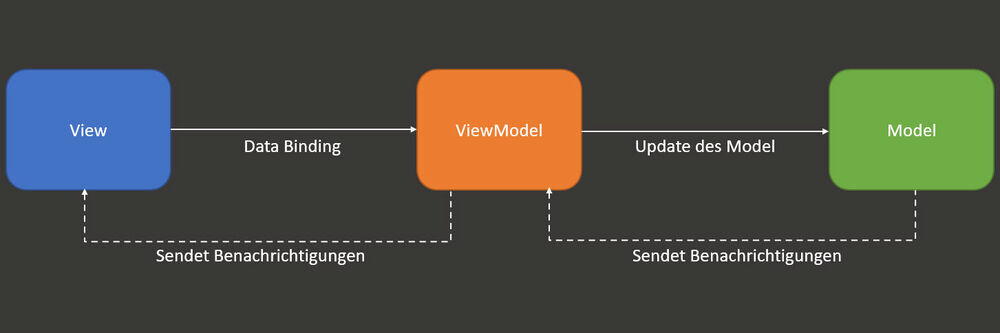
\includegraphics[width=1.0\linewidth]{./images/MVVM.png}
		\caption{MVVM \cite{MVVMKraus}}
		\label{fig:MVVM}
	\end{figure}
	\begin{itemize}
		\item \textbf{Model: } Hier werden Daten aus einer Datenquelle angefordert und bearbeitet.
		\item \textbf{View: } In der View wird die Graphische Oberfläche definiert. Zur Darstellung von Daten nutzt Sie ViewModel, welches Informationen für die View zur Vergügung stellt.
		\item \textbf{ViewModel: } Das ViewModel ähnelt dem Controller von MVC und stellt die Verbindung zwischen Model und View her. Hier wird die Logik, was bei Änderungen an der Benutzeroberfläche passieren soll, geschehen soll implementiert. ViewModel holt sich von Model Daten, welche die View für Darstellungszwecke benötigt. \cite{MVVMKraus} \cite{troelsen2022pro}
	\end{itemize}
	Auf die Verbindung wischen den einzelnen Komponenten mit Data Binding wird im folgenden unter Entwurfsmuster eingegangen.\\
	\textbf{Entwurfsmuster}\\
	Nach \cite{ArchitekturmusterGoll} bieten sich für die MVC-Architektur und somit auch für die MVVM-Architektur mehrere Entwurfsmuster an. Am geläufigsten ist das Beobachter-Muster (engl. Observer-Pattern). Weitere Entwurfsmuster sind das Strategie-Muster und das Kompositum-Muster. \cite{ArchitekturmusterGoll}. Das Beobachter-Muster wird häufig in der Literatur empfohlen und kommt auch in der WPF-Anwendung roboTools umgesetzt durch sogenannte Datenbindung (engl. Data Binding) zum Einsatz. Daher fällt die Entscheidung bei der zu entwerfenden WPF-Anwendung ebenso auf MVVM mit Beobachter-Muster. Die beobachtende Komponente überwacht hierbei eine andere Komponenten. Ändert sich etwas an dem beobachtenden Objekt (wie z.B. ein Tastendruck) erkennt dies der Beobachter und kann in Folge dessen eine definierte Aktion ausführen. \cite{ArchitekturmusterGoll} Die Verbindung zwischen View und ViewModel, sowie zwischen ViewModel und Model wird mit Hilfe von Datenbindung umgesetzt. Die Datenbindung gibt sozusagen Daten zwischen einzelnen Komponenten weiter.\\
	\textbf{Adaption der Anwendung auf Architektur- und Entwurfsmuster}\\
	Um die Komponenten der zu entwerfenden Software zu definieren, müssen die Anwendungen, die im UML-Diagramm (vgl. Abbildung \ref{fig:UML_Use_Case_WPF}) definiert wurden auf das Entwurfsmuster aufgeteilt werden. Ebenso müssen die Klassen für die zu entwerfende WPF-Anwendung in C\# definiert werden. Gemäß WVVM werden in der View (gemäß unternehmensinternem Standard als "MainWindow" bezeichnet)
	die Grafik des Programms festgelegt. Hier müssen sowohl der Prokollschreiber der Systemereignisse, sowie Diagramme zur Darstellung der Prozessdaten definiert werden. In der View soll jedoch keine Logik umgesetzt und der Code auf ein Minimum begrenz werden. Im Model hingegen erfolgt gemäß MVVM die Datenhaltung und Datenverarbeitung. Hier werden Daten über die TCP/IP-Verbindung empfangen und gesendet, sowie die Daten abgespeichert. Das ViewModel (unternehmensintern als MainViewModel bezeichnet) verkünpft die View und das Model. So soll auf Knopfdruck in der View, Prozessdaten aus dem Model ausgelesen und in der View dargestellt werden. Die Logik hierfür erfolgt in dem ViewModel (hier: MainViewModel). Für den Entwurf der WPF-Anwendung bietet sich daher folgende Klassenaufteilung an, welche nachfolgend in einem UML-Klassendiagramm dargestellt ist (vgl. Abbildung \ref{fig:UMLKlassenWPF}). Diese Klassen sind in der Umsetzung mit C\# zu implementieren.
	\begin{figure}
		\begin{tikzpicture}
			\begin{umlpackage}{ViewModel}
				\umlclass[name=viewModel, x=0]{MainViewModel}{
				}{
					+ ploteDaten() : void
				}
			\end{umlpackage}
			
			\begin{umlpackage}{View}
				\umlclass[name=view, x=8]{MainWindow}{
					- Graphik: \\
					- Zustand Button: \\
					- Protokollschreiber:
				}{
					
				}
			\end{umlpackage}
			
			\begin{umlpackage}{Model}
				\umlclass[name=com, x=0, y=-6]{Communicator}{
					- IP-Adresse : float \\
					- Verbundene Clients: List Client
				}{
					+ sende Nachricht() : void \\
					+ empfange Nachricht() : void \\
					+ Interpretiere Datentelegramm(): void \\
					+ Speichere Daten(): void \\
					+ Interpretiere Systemereignis\\-Telegramm(): void \\
					+ Speichere Systemereignisse(): void \\
					+ Sende Aktualisierungs-Telegram \\Schwere Systemereignis(): void\\
					+ Sende Positionsdaten(): void
				}
				
				\umlclass[name=robot, x=8, y=-6]{Robot}{
					- Temperatur: int \\
					- Fehler: bool \\
					- Schwere Systemerigniss: int
				}{
					
				}
			\end{umlpackage}
			
			
			% Verbindungslienie zwischen SPS und Roboter mit Multiplicitäten
			\umlassoc[pos=0.5]{MainViewModel}{MainWindow}
			\umlassoc[pos=0.5]{MainViewModel}{Communicator}
			\umlassoc[pos=0.5]{Communicator}{Robot}
			
		\end{tikzpicture}
		\caption{UML-Klassendiagramm WPF-Anwendung}
		\label{fig:UMLKlassenWPF}
	\end{figure}
	
	\chapter{Design und Implementierung}
	Design: Vergleich von Lösungsbausteinen (z.B. Vergleich Softwarebibliotheken) und Auswahl) auf Basis von Anforderungen und Recherche. Wissenschaftliche Bewertungskriterien nötig. Harvey-Diagramm.
	
	Neben grundlegenden Entwurfsentscheidungen wird die Beschreibung einzelner Komponenten detailiert. Für komplexe Komponenten UML-Klassendiagramm
	Definition Schnittstelle zwischen den Komponenten und Kommunikation in Form von Sequenzdiagramm
	
	
	Implementierung
	- Programmierung erfolgt gemäß den in Softwarespezifikation und entwurf festgelegten Randbedingungen, Kommentierung von Source Code ist essentiell. Gemäß bestehenden Standards (z.B. xdoc)
	- Generierung einer HTML-Hilfe aus den Kommentaren des Source-Codes z.b. durch Doxygen
	- Entwicklung erfolgt unter Git
	- Einheitliche Konventionen für das Schreiben des Quellcodes: Coding Conventions!
	\section{Stäubli-Roboter in VAL3}
	
	\subsection{EtherCAT}
	
	\subsection{TCP/IP}
	Für die Implementierung der TCP/IP-Verbindung auf dem Controller des Stäubli-Roboters muss in der SRS eine Socket-Verbindung angelegt werden. Hierzu wird in der E/A-Verwaltung ein Client angelegt, welcher die IP-Adresse und den Port des Servers zugewiesen bekommt. Darüber hinaus wird ein sogenannter Timeout von 0 s gesetzt. Bei einem Timeout von 0 wird auf den Vorgang, welcher ein Lesen oder Schreiben sein kann gewartet. Bei einem Timeout kleiner 0 wird hingegen nicht bis zur Ausführung des Vorgangs gewartet. Be einem Timeout größer 0 wird hingegen eine gewisse Zeit gewährt, bis zu dieser der Timeout durchgeführt werden kann. Die Nachricht soll in diesem Fall jedoch direkt gelesen oder geschrieben werden, weshalb kein Spielraum im Rahmen des Timeouts gewährt wird. \cite{VAL3} Die Socket-Verbindung wird als E/A-Verbindung in VAL3 betrachtet, weshalb eine globale Variable mit dem Namen des Clients angelegt werden kann und hierüber auch gelesen und beschrieben werden kann. Die Socket-Verbindung wird nur dann erstellt, wenn sie ihm Rahmen des Programmablaufs z.B. durch die Befehle sioSet und sioGet benötigt wird. Der Client versucht dann eine Verbindung zum Server aufzubauen.   usepackage{ffcode}\\
	num sioGet(sio siInput, num\& nData[])\\
	Diese Funktion schreibt ein gelesenes Zeichen oder einen gelesen Array von Zeichen von siInput in das Array nData. Als Rückgabewert dient die Anzahl der gelesenen Zeichen.	
	num sioSet(sio siOutput, num\& nData[]) \\
	Mit dieser Funktion kann in VAL3 die zu übermittelnde Nachricht nData versendet werden, indem der E/A-Verbindung siOutput die Nachricht zugewiesen wird. Zurückgegeben wird die Anzahl der geschriebenen Zeichen oder "-1" im Falle des Timeouts. \\
	Das Versenden von Nachrichten erfolgt über einen Byte-Array, das heißt durch die Aneinanderreihung mehrerer Bytes. Folglich muss die zu versendete Nachricht in einen Byte-Array umgewandelt werden und beim Empfangen muss der Byte-Array interpretiert werden.\\
	num toBinary(num nValue[], num nValueSize, string sDataFormat, num\& nDataByte[])\\
	Diese Funktion wandelt einen numerischen Wert, welcher das Datenformat sDataFormat besitzt in einen Byte-Strom und speichert diesen im Array nDataByte. Über das Datenformat wird beispielsweise angegeben ob es sich um einen Gleitkommawert handelt, ob ein Vorzeichen vorliegt und ob das Little-Endian oder das Big-Endian-Format angewandt wird. Mit nDataSize kann die Anzahl der zu kodierenden Zeichen beschränkt werden.\\
	num fromBinary(num nDataByte[], num nDataSize, string sDataFormat, num\& nValue[])\\
	Umgekehrt ermöglicht diese Funktion, einen empfangen Byte-Array in numerische Werte zu konvertieren. Das Ergebnis im Datenformat nDataFormat wird in nValue gespeichert. Die Anzahl der zu decodierenden Bytes wird festgelegt durch nDataSize, wenn nicht alle Bytes des Eingangs-Array nDataByte decodiert werden sollen.
	
	\section{WPF-Anwendung}
	Wie in Stand der Technik. WPF, C, VisualStudio and DevOps.
	
	\subsection{Architektur}
	
   	\subsection{TCP/IP-Server}
   	
   	\subsection{Daten-Logger}
   	
   	\subsection{Graphen}
   	
   	
   	\chapter{Validierung}
   	
   	\chapter{Ausblick und Fazit}
   	
   	\backmatter
   	
   	
   	\cleardoublepage
   	\listoffigures
   	\cleardoublepage
   	\listoftables
   	\cleardoublepage
   	
   	\cleardoublepage
   	\printbibliography
   	
   	% Acronyms   	
   	% Appendix, if needed:
   

\end{document}